%%%%%%%%%%%%%%%%%%%%%%%%%%%%%%%%%%%%%%%%%%%%%%%%%%%%%%%%%%%%%%%%%%%%%%%%%%%%%%%
%% Descr:       Vorlage für Berichte der DHBW-Karlsruhe
%% Author:      Prof. Dr. Jürgen Vollmer, vollmer@dhbw-karlsruhe.de
%% $Id: bericht.tex,v 1.19 2016/03/16 16:59:41 vollmer Exp $
%%  -*- coding: utf-8 -*-
%%%%%%%%%%%%%%%%%%%%%%%%%%%%%%%%%%%%%%%%%%%%%%%%%%%%%%%%%%%%%%%%%%%%%%%%%%%%%%%

\documentclass[
   ngerman          % neue deutsche Rechtschreibung
  ,a4paper          % Papiergrösse
% ,twoside          % Zweiseitiger Druck (rechts/links)
% ,10pt             % Schriftgrösse
% ,11pt
 ,12pt
  ,pdftex
%  ,disable         % Todo-Markierungen auschalten
%  ,ngerman
]{scrreprt}

\usepackage[onehalfspacing]{setspace} %Zeilenabstand
%\usepackage[doublespacing]{setspace} %Zeilenabstand

% Bitte die Codierung Ihrer Dateien auswählen:
% \usepackage[latin1]{inputenc}    % Für UNIX mit ISO-LATIN-codierten Dateien
% \usepackage[applemac]{inputenc}  % Für Apple Mac
% \usepackage[ansinew]{inputenc}   % Für Microsoft Windows
\usepackage[utf8]{inputenc}        % UTF-8 codierte Dateien
                                   % Dieses Dokument ist unter Unix erstellt, daher
                                   % wird diese Input-Codierung benutzt.

\usepackage{bericht}
\usepackage[german,english]{babel}
%\selectlanguage{english}

\usepackage{amsmath}
\usepackage[binary-units = true]{siunitx}
\sisetup{
%  locale = DE ,
  per-mode = symbol
}
\DeclareSIUnit{\sqrthz}{\ensuremath{\sqrt{\text{\hertz}}}}
\DeclareSIUnit{\voltnoise}{\volt\per\sqrthz}
\DeclareSIUnit{\decibelm}{\ensuremath{\text{dBm}}}
\DeclareSIUnit{\decibeli}{\ensuremath{\text{dBi}}}

\usepackage{xfrac}
\usepackage{extarrows}
\usepackage{xspace}

\graphicspath{{Bilder/}} %Setting the graphicspath
% ============= Dokumentinformationen =======================================

%\newcommand{\Bericht}{Laborbericht}
\newcommand{\Titel}{Master-Thesis}
\newcommand{\Was}{Untersuchung und Beurteilung der OTA-RSE-Messmethode im Kontext von 3GPP 5G FR2}
\newcommand{\WasEng}{Assessment of OTA RSE Measurement Method in the Context of 3GPP 5G FR2}
\newcommand{\Referent}{Prof. Dr.-Ing. Manfred Litzenburger}
\newcommand{\Korreferent}{Prof. Dr.-Ing. Hans Sapotta}
\newcommand{\Betreuer}{Dipl.-Ing. Heinz Mellein}
\newcommand{\Autor}{Fabian Michaelsen}
\newcommand{\UNI}{Hochschule Karlsruhe - Technik und Wirtschaft}
\newcommand{\firma}{Rohde \& Schwarz GmbH \& Co. KG}
\newcommand{\Studiengang}{Fakultät für Elektro- und Informationstechnik}
\newcommand{\MatrikelNummer}{62032}
\newcommand{\ThesisNummer}{300}
\newcommand{\Zeitraum}{01.05.2019 - 31.10.2019}
% Wird auf dem Deckblatt in der Erklärung benutzt

\newcommand{\abs}[1]{\ensuremath{\left\vert#1\right\vert}}

%%%%%%%%%%%%%%%%%%%%%%%%%%%%%%%%%%%%%%%%%%%%%%%%%%%%%%%%%%%%%%%%%%%%%%%%%%%%%%%%%%%%%

\hypersetup{%%
  pdfauthor={\Autor},
  pdftitle={\Titel},
  pdfsubject={\Was}
}

%%%%%%%%%%%%%%%%%%%%%%%%%%%%%%%%%%%%%%%%%%%%%%%%%%%%%%%%%%%%%%%%%%%%%%%%%%%%%%%

% Wenn \includeonly{..} benutzt wird, werden nur diese Kaptitel ausgegeben.
%\includeonly{
%  abk
% ,adaption
%}

%%%%%%%%%%%%%%%%%%%%%%%%%%%%%%%%%%%%%%%%%%%%%%%%%%%%%%%%%%%%%%%%%%%%%%%%%%%%%%%

% Benutzt man das "biblatex"-Paket, dann muß das hier stehen:
% siehe auch die mit BIBLATEX markierten Zeilen in bericht.sty
\bibliography{literatur}

\begin{document}
%%%%%%%%%%%%%%%%%%%%%%%%%%%%%%%%%%%%%%%%%%%%%%%%%%%%%%%%%%%%%%%%%%%%%%%%%%%%%%%
\pagenumbering{roman}

\begin{titlepage}

\begin{singlespace}
\begin{center}
\begin{singlespace}
\Large \Titel\\[1.2cm]
\end{singlespace}
\begin{spacing}{2}
{\Huge\scshape \Was}\\
{\Large \WasEng}\\[0.6cm]
\end{spacing}
\end{center}
\end{singlespace}

\begin{flushleft}
	\begin{center}
		
\includegraphics[width=12cm]{HSKA_Logo_Hska_Logo.pdf}
		%\includegraphics[width=12.7cm]{8_2_3_3_Bild1.JPG}
	\end{center}
\end{flushleft}

\begin{singlespace}
\begin{center}
%\vspace*{-2cm}
{\large \Studiengang}\\[0.5cm]
{\large von}\\[0.5cm]
{\large\bfseries \Autor}\\[0.5cm]
\vfill
\end{center}
\begin{tabular}{l@{\hspace{2cm}}l}
Matrikelnummer	                 & \MatrikelNummer		\\
Thesis Nummer		& \ThesisNummer \\
Zeitraum	&	\Zeitraum \\ \\
Referent der Hochschule	 & \Referent		\\
Korreferent der Hochschule	 & \Korreferent		\\ \\
Betreuer am Arbeitsplatz	 & \Betreuer		\\
Firma	 & \firma		\\
\end{tabular}
\end{singlespace}
\end{titlepage}


%\vspace{0cm}

%\begin{center}
%
%	\Huge{
%		\textbf{\Vorlesung}} \\[0.5cm]
%	\huge{
%		\textbf{{\Versuch}}\\[7.0cm]
%		}
%	\normalsize{
%		}
%	\normalsize{
%		\textbf{{\Versuchstermin}}\\[3.0cm]
%	}
%	
%	\small{
%		\textbf{\firma} \\
%	}
 %   \small{
	%	\textbf{\studiengang} \\
	%	}
	

%\end{center}
%
%}



%%%%%%%%%%%%%%%%%%%%%%%%%%%%%%%%%%%%%%%%%%%%%%%%%%%%%%%%%%%%%%%%%%%%%%%%%%%%%%%

% Nur für Bachelorarbeiten einfügen:
\setlength{\parindent}{0pt}
%%%%%%%%%%%%%%%%%%%%%%%%%%%%%%%%%%%%%%%%%%%%%%%%%%%%%%%%%%%%%%%%%%%%%%%%%%%%%%%
%% Descr:       Vorlage für Berichte der DHBW-Karlsruhe, Erklärung
%% Author:      Prof. Dr. Jürgen Vollmer, vollmer@dhbw-karlsruhe.de
%% $Id: erklaerung.tex,v 1.6 2016/03/16 12:51:09 vollmer Exp $
%% -*- coding: utf-8 -*-
%%%%%%%%%%%%%%%%%%%%%%%%%%%%%%%%%%%%%%%%%%%%%%%%%%%%%%%%%%%%%%%%%%%%%%%%%%%%%%%

% In Bachelorarbeiten muss eine schriftliche Erklärung abgegeben werden.
% Hierin bestätigen die Studierenden, dass die Bachelorarbeit, etc.
% selbständig verfasst und sämtliche Quellen und Hilfsmittel angegeben sind. Diese Erklärung
% bildet das zweite Blatt der Arbeit. Der Text dieser Erklärung muss auf einer separaten Seite
% wie unten angegeben lauten.

\newpage
\thispagestyle{empty}
%\begin{framed}
\begin{center}
\Huge\emph{Eidesstattliche Erklärung}
\end{center}
\medskip
\noindent
Ich versichere hiermit, dass ich meine \Titel\ mit
dem Thema: \glqq \Was \grqq{ }selbständig verfasst und keine anderen als die angegebenen Quellen und Hilfsmittel benutzt habe.

\vspace{3cm}
\noindent
\underline{\hspace{6cm}}\hfill\underline{\hspace{6cm}}\\
Ort\hspace{2.5cm}Datum\hfill Unterschrift\hspace{3.8cm}
%\end{framed}

\vfill
%\emph{Sofern von der Ausbildungsstätte ein Sperrvermerk gewünscht %wird, ist folgende Formulierung
%zu verwenden:}
%\begin{framed}
%\begin{center}
%\Large\bfseries Sperrvermerk
%\end{center}
%\medskip
%\noindent
%Der Inhalt dieser Arbeit darf weder als Ganzes noch in Auszügen %Personen
%auerhalb des Prüfungsprozesses und des Evaluationsverfahrens %zugänglich gemacht
%werden, sofern keine anders lautende Genehmigung der %Ausbildungsstätte vorliegt.
%\end{framed}

%%%%%%%%%%%%%%%%%%%%%%%%%%%%%%%%%%%%%%%%%%%%%%%%%%%%%%%%%%%%%%%%%%%%%%%%%%%%%%%
\endinput
%%%%%%%%%%%%%%%%%%%%%%%%%%%%%%%%%%%%%%%%%%%%%%%%%%%%%%%%%%%%%%%%%%%%%%%%%%%%%%%

\newpage


\newpage
\thispagestyle{empty}
%\begin{framed}
\begin{center}
\Huge\emph{Kurzfassung}
\end{center}
\medskip
\noindent

Der kommende Mobilfunkstandard 5G NR, der von 3GPP entwickelt wird, nutzt Frequenzen im Millimeterwellenbereich.
Bei diesen kurzen Wellenlängen sind herkömmliche Testmethoden, die Kabelkonnektoren in der Benutzerausrüstung benötigen, aufgrund des hohen Integrationsgrades moderner aktiver Antennensysteme impraktikabel.
Daher müssen in Zukunft Konformitätstests und Störstrahlungsmessungen für den Millimeterwellenbereich über die Luft, unter Verwendung der Metrik TRP, durchgeführt werden.
Die Grenzwerte für elektromagnetische Emissionen sind im Vergleich zwischen der Europäischen Union und den Vereinigten Staaten von Amerika dargelegt.
Erst werden theoretische Hintergründe in den erforderlichen Bereichen der Antennentheorie, räumlicher Abtastung, sphärischer Abtastnetze, sphärischer Quadraturen, Stochastik und Regression erklärt.\\

Anschließend folgt die Untersuchung aller Aspekte von TRP-Messungen über die Luft.
Angefangen bei der Messkammerauswahl, um eine ausreichende Dynamik zu ermöglichen und Quiet Zone zu erreichen, der Kalibrierung eines Messplatzes, der Bewertung des Dynamikbereichs anhand des Link Budget und der Auswahl der idealen Detektoreinstellung für das verwendete Messgerät.
Anschließend folgt die Erarbeitung eines konkreten Vorschlags zur idealen Durchführung der TRP-Messung.
Einerseits wird der minimal erforderliche Messabstand und die ideale Messantenne um eine einfache Messung durch kurze Messabstände, der über die Luft TRP-Messung, untersucht.
Hierzu folgt die Entwickelung und Durchführung einer Simulation der getesteten Antenne, der Messantenne und des Messradius.
Mit verschiedenen Parametersätzen wird die Tendenz ermittelt, dass Messantennen mit geringerer Direktivität bei gleichem Messabstand weniger Fehler verursachen. Dies wird durch eine Messkampagne bestätigt.\\

Andererseits werden der sphärische Abtasttyp und die Messdichte mithilfe einer statistischen Simulation untersucht, welche rechteckige Antennenarrays mit zufälligen Steering-Vektoren verwendet.
Es ist wichtig, einfach realisierbare Abtastungen mit so wenig Punkten auf der Kugel wie möglich zu kombinieren, um in kürzester Zeit eine bestimmte Genauigkeit der TRP-Messung zu erzielen.
Hier hat sich der, in dieser Arbeit entwickelte, Referenzwinkelkorrekturfaktor als die optimale Methode erwiesen, um einen öffnungsunabhängigen Messfehler mit einer gleichförmigen sphärischen Abtastung mit ausgedünnter Abtastung an den Polen, zu erreichen.
Dies wurde durch eine Regression bewiesen.



\newpage
\thispagestyle{empty}
%\begin{framed}
\begin{center}
\Huge\emph{Abstract}
\end{center}
\medskip
\noindent

You schould measure \ac{RSE} to be sure of not disturbing others!



\newpage
\thispagestyle{empty}
%\begin{framed}
\begin{center}
\Huge\emph{Vorwort}
\end{center}
\medskip
\noindent

Hier möchte ich allen danken, die mich bei dieser Arbeit fachlich und persönlich unterstützt haben. Mein besonderer Dank gilt meinem Betreuer bei Rohde \& Schwarz in München Heinz Mellein, der das interessante Thema bereitstellte und mich bei der Durchführung immer sehr freundlich, kompetent und unkompliziert betreut hat. Außerdem möchte ich meinen Kollegen Johannes Köbele und Gerhard Hamberger danken, ohne deren gute Ratschläge und allgemeine Unterstützung diese Arbeit in dieser Form nicht möglich gewesen wäre. Ich möchte auch Ahmed Ezzouhri und Simon Lachner für die Unterstützung bei langwierigen Messkampagnen danken. Auch danke ich meinen betreuenden Professoren der Hochschule Karlsruhe Manfred Litzenburger und Hans Sapotta für ihre zurückhaltende, freundliche und kompetente Unterstützung. Vor allem danke ich der Kantine von Rohde und Schwarz für die gute und günstige Verpflegung und allen neuen Freunden in München für die tolle und abwechslungsreiche Zeit hier.

\begin{flushright}
Fabian Michaelsen\\
September 2019\\
München
\end{flushright}


\tableofcontents           % Inhaltsverzeichnis hier ausgeben
\listoffigures             % Liste der Abbildungen
\listoftables              % Liste der Tabellen
%\lstlistoflistings         % Liste der Listings
%\listofequations           % Liste der Formeln

% Jetzt kommt der "eigentliche" Text
%%%%%%%%%%%%%%%%%%%%%%%%%%%%%%%%%%%%%%%%%%%%%%%%%%%%%%%%%%%%%%%%%%%%%%%%%%%%%%
%% Descr:       Vorlage für Berichte der DHBW-Karlsruhe, Datei mit Abkürzungen
%% Author:      Prof. Dr. Jürgen Vollmer, vollmer@dhbw-karlsruhe.de
%% $Id: abk.tex,v 1.3 2016/03/16 12:21:40 vollmer draft $
%% -*- coding: utf-8 -*-
%%%%%%%%%%%%%%%%%%%%%%%%%%%%%%%%%%%%%%%%%%%%%%%%%%%%%%%%%%%%%%%%%%%%%%%%%%%%%%%

\chapter*{List of Abbreviations}                   % chapter*{..} -->   keine Nummer, kein "Kapitel"
						         % Nicht ins Inhaltsverzeichnis
% \addcontentsline{toc}{chapter}{Akürzungsverzeichnis}   % Damit das doch ins Inhaltsverzeichnis kommt

% Hier werden die Abkürzungen definiert
\begin{acronym}[FIAFTA]
  % \acro{Name}{Darstellung der Abkürzung}{Langform der Abkürzung}
 \acro{Abk}[Abk.]{Abkürzung}

 % Folgendes benutzen, wenn der Plural einer Abk. benöigt wird
 % \newacroplural{Name}{Darstellung der Abkürzung}{Langform der Abkürzung}
 \newacroplural{Abk}[Abk-en]{Abkürzungen}

 \acro{H2O}[\ensuremath{H_2O}]{Di-Hydrog-Monoxid}

 % Wenn neicht benutzt, erscheint diese Abk. nicht in der Liste
 \acro{NUA}{Not Used Acronym}
 
 \acro{3GPP}{3rd Generation Partnership Project}
 \acro{5G}{Fifth Generation mobile communication}
 \acro{AAS}{Active Antenna System}
 \acro{AC}{Anechoic Chamber}
 \acro{ANSI}{American National Standards Institute}
 \acro{ATS}{Antenna Test System}
 \acro{CATR}{Compact Antenna Test Range}
 \acro{CC}{Clenshaw–Curtis}
 \acro{CDG}{Constant Density Grid}
 \acro{CEPT}{European Conference of Postal and Telecommunications Administrations}
 \acro{CrefA}{Correction Factor Reference Angle}
 \acro{CSSG}{Constant Step Size Grid}
 \acro{DANL}{Displayed Average Noise Level}
 \acro{DUT}{Device Under Test} 
 \acro{EBW}{Emission Bandwidth}
 \acro{EIRP}{Equivalent Isotropic Radiated Power}
 \acro{EM}{Electro Magnetic}
 \acro{EMC}{Electro Magnetic Compatibility}
 \acro{ETSI}{European Telecommunications Standards Institute}
 \acro{EU}{European Union}
 \acro{FCC}{Federal Communications Commission}
 \acro{FF}{Far-Field}
 \acro{FFT}{Fast Fourier Transformation}
 \acro{FR2}{Frequency Range two}
 \acro{FSPL}{Free Space Path Loss}
 \acro{IEEE}{Institute of Electrical and Electronics Engineers}
 \acro{ITU}{International Telecommunication Union}
 \acro{LB}{Link Budget}
 \acro{MIMO}{Multiple In Multiple Out}
 \acro{mmW}{milli-meter Wave}
 \acro{NF}{Near-Field}
 \acro{NR}{New Radio}
 \acro{OATS}{Open Area Test Site}
 \acro{OBW}{Occupied Bandwidth}
 \acro{OEM}{Original Equipment Manufacturer}
 \newacroplural{OEM}[OEMs]{Original Equipment Manufacturer}
 \acro{OOBE}{Out Of Band Emission}
 \acro{OTA}{Over The Air}
 \acro{PM}{Pattern Multiplication}
 \acro{QZ}{Quiet zone}
 \acro{RBW}{Resolution Bandwidth}
 \acro{RF}{Radio Frequency}
 \acro{RMS}{Root Mean Square}
 \acro{RS}[R\&{}S]{Rohde \& Schwarz GmbH \& Co. KG}
 \acro{RSE}{Radiated Spurious Emission} 
 \acro{RVC}{Reverberation Chamber}
 \acro{SE}{Spurious Emission}
 \acro{SF}{Sparsity Factor}
 \acro{SGH}{Standard Gain Horn}
 \acro{TMP}{Total Measurement Power}
 \acro{TRP}{Total Radiated Power}
 \acro{TSP}{Travelling Salesman Problem}
 \acro{UE}{User Equipment}
 \acro{UnE}{Unwanted Emission}
 \acro{USA}{United States of America}
 \acro{VNA}{Vector Network Analyzers}
 \acro{VSG}{Vector Signal Generator}


\end{acronym}              % Abkürzungsverzeichnis
\pagenumbering{arabic}

%\include{src/Einleitung}
\chapter{Introduction}

In this chapter the motivation and aim of this work is phrased. Furthermore the current emission limits and the necessary terms are presented.

\section{Motivation}

\ac{3GPP} \ac{5G} is occupying \acp{mmW} in \ac{FR2} with frequencies $\ge\SI{28}{\giga\hertz}$ \cite{trp}. With this development big and highly integrated  \acp{AAS} will be needed. That makes the conducted conformance test approach with antenna connectors in the \ac{UE} impossible. The equivalent metric to conducted measurements for \ac{RSE} is now \ac{TRP} and the measurement is carried out \ac{OTA}.

%Higher frequencies imply shorter wavelengths. Multi-antenna arrays at mmWave frequencies will help overcome signal propagation issues and deliver directional antennas with higher gain. With shorter wavelengths, antenna elements can be spaced more tightly, resulting in extremely compact arrays. Many vendors even opt to develop arrays that integrate into ICs. Of course, highly integrated ICs have no place to probe and no place to put connectors. A consequence of this integration is it has become impractical to use traditional RF connectors between the radio circuit and the antenna, bringing the need for OTA tests. https://www.testandmeasurementtips.com/why-5g-is-going-to-over-the-air-testing-faq/

\section{Aim}

The aim of this work is to find an optimal solution for conformance  \ac{TRP}-measurements using \acp{AC}. In dependence of the dimension of the \ac{DUT} an ideal grid and measurement distance for a wanted precision shall be found. To achieve that, theoretical knowledge shall be projected on simulations and the outcome shall be proofed in real measurements.

\section{Legal Emission Limits}
\label{sec:legem}

In this section the official \ac{EM} emission limits are acknowledged by the example of the regulation in the \ac{USA} and the \ac{EU}. The \ac{ITU} provides a recommendation \cite{seitur} about the emission limits for the national regulators. These regulators, in the \ac{EU} the \ac{CEPT} and in the \ac{USA} the \ac{FCC}, publish with the help of dedicated standardisation organisations, e.g. \ac{ETSI} (\ac{EU}), \ac{ANSI} (\ac{USA}) or other \acp{SDO}, limits which become law; \cite{ceptercrec}, \cite{ansi}. The \ac{3GPP}, the \ac{IEEE} or other \acp{SDO} develop a new telecommunication standard and adopt to this laws.\\
To quantify emission limits the following terms are declared regarding \cite{seitur} and \cite{ctiaat}:

\begin{itemize}
\item An \textbf{\acf{UnE}} consists of \ac{SE} and \ac{OOBE}.
\item A \textbf{\acf{SE}} is an emission on a frequency, or frequencies, which are outside the necessary bandwidth and the level of which may be reduced without affecting the corresponding transmission of information. \acl{SE} include harmonic
emissions, parasitic emissions, intermodulation products and frequency conversion products but exclude \ac{OOBE}.
\item An \textbf{\acf{OOBE}} is an emission on a frequency or frequencies immediately outside the necessary bandwidth which results from the modulation process, excluding \aclp{SE}.
\item The \textbf{\acf{OBW}} is the bandwidth wherein $\SI{99}{\percent}$ of the power is radiated.
\item The \textbf{\acf{EBW}} is used by the \ac{FCC} and describes a bandwidth which is surrendered out of that tow points in the spectra lying $\SI{26}{\decibel}$ under the power of the \ac{OBW}. 
\item \textbf{\acf{TRP}} is the \ac{OTA} equivalent for measuring connected and describes all power radiated by a device. It is the average spherical \ac{EIRP}.
\end{itemize}


In table \ref{tab:legusa} the emission limits from \cite{ceptercrec}, \cite{ansi} and \cite{fcc} are summarized. The used terms are illustrated in fig. \ref{fig:sem}.

\begin{table}
\centering
\caption{Legal Emission Limits}
\label{tab:legusa}
\begin{tabular}{|c|c|c|c|}
\hline
$f_c$  &  $f_l$ & $f_h$ & $p_e$ \\\hline
\multicolumn{4}{|c|}{\textbf{USA}} \\\hline
$\SI{9}{\kilo\hertz}-\SI{10}{\giga\hertz}$ & $\SI{9}{\kilo\hertz}$ & $10f_c\ \text{or}\ \SI{40}{\giga\hertz}$ & $\SI{-13}{\decibelm\per\mega\hertz}$ \\\hline
$\SI{10}{\giga\hertz}-\SI{30}{\giga\hertz}$ & $\SI{9}{\kilo\hertz}$ & $5f_c\ \text{or}\ \SI{100}{\giga\hertz}$ & $\SI{-13}{\decibelm\per\mega\hertz}\ \text{or}\ 1\% \text{EBW}$ \\\hline
$\SI{30}{\giga\hertz}-\dots$ & $\SI{9}{\kilo\hertz}$ & $5f_c\ \text{or}\ \SI{200}{\giga\hertz}$ & $\SI{-13}{\decibelm\per\mega\hertz}\ \text{or}\ 1\% \text{EBW}$ \\\hline
\multicolumn{4}{|c|}{\textbf{EU}} \\\hline
$\SI{9}{\kilo\hertz}-\SI{100}{\mega\hertz}$ & $\SI{9}{\kilo\hertz}$ & $\SI{1}{\giga\hertz}$ & $\SI{-36}{\decibelm\per \SI{100}{\kilo\hertz}}$ \\\hline
$\SI{100}{\mega\hertz}-\SI{300}{\mega\hertz}$ & $\SI{9}{\kilo\hertz}$ & $10f_c$ & $\SI{-36}{\decibelm\per \SI{100}{\kilo\hertz}}$ \\\hline
$\SI{300}{\mega\hertz}-\SI{600}{\mega\hertz}$ & $\SI{30}{\mega\hertz}$ & $\SI{3}{\giga\hertz}$ & $\SI{-36}{\decibelm\per \SI{100}{\kilo\hertz}}$ \\\hline
$\SI{600}{\mega\hertz}-\SI{1}{\giga\hertz}$ & $\SI{30}{\mega\hertz}$ & $5f_c$ & $\SI{-36}{\decibelm\per \SI{100}{\kilo\hertz}}$ \\\hline
$\SI{1}{\giga\hertz}-\SI{5.2}{\giga\hertz}$ & $\SI{30}{\mega\hertz}$ & $5f_c$ & $\SI{-30}{\decibelm\per\mega\hertz}$ \\\hline
$\SI{5.2}{\giga\hertz}-\SI{7.25}{\giga\hertz}$ & $\SI{30}{\mega\hertz}$ & $\SI{26}{\giga\hertz}$ & $\SI{-30}{\decibelm\per\mega\hertz}$ \\\hline
$\SI{7.25}{\giga\hertz}-\dots$ & $\SI{30}{\mega\hertz}$ & $2f_c$ & $\SI{-13}{\decibelm\per\mega\hertz}\ \text{and}\ \SI{-10}{\decibelm\per \SI{100}{\kilo\hertz}}$ \\\hline
\end{tabular}
\end{table}

\begin{figure}
\centering
\def\svgwidth{0.9\textwidth}
\input{Bilder/EmissionMask.pdf_tex}
\caption{Spurious Emissions Mask}
\label{fig:sem}
\end{figure}









\chapter{Theoretical Background}

This chapter will give a brief overview about the underlying theoretical background in the fields of antenna theory, spatial sampling, will introduce quadrature methods for deriving the \ac{TRP} out of spherical \ac{EIRP} data and will establish the needed stochastic for the used statistic.

\section{Antenna Field Regions}

\begin{figure}[H]
\centering
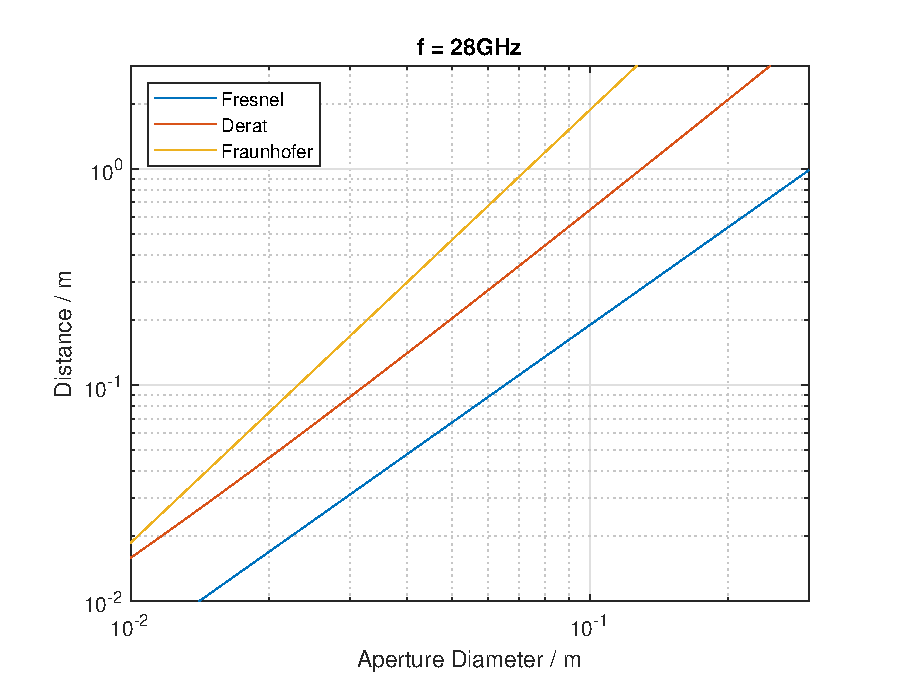
\includegraphics[width=0.6\textwidth]{Matlab/AntennaFieldRegions.eps}
\caption{Antenna field regions overview}
\label{fig:antennafieldreg}
\end{figure}

There are three commonly known antenna field regions, the reactive \ac{NF}, the radiating \ac{NF} and the \ac{FF}, divided by two boundaries, the Fresnel distance (blue) and the Fraunhofer distance (yellow). These distances are shown in figure \ref{fig:antennafieldreg}, where the aperture diameter of an arbitrary antenna is on the x-axis and the distance form it is on the y-axis. The third line, the Derat distance (red), was introduced by Benoit Derat in \cite{8393926}.\\
\ac{FF}-distance and \ac{NF}-distance are derivable from the phase fluctuation due to the maximum diameter of the antennas aperture \cite{7942128} in a distance $r$ from the antennas phase center. The phase fluctuation is given by the different length of $r$ and $R$, as you can see in figure \ref{fig:arbaperturexy}. The maximum runtime difference is found at the minimum radius of the circle enclosing the aperture at $\sfrac{D}{2}$. The field boundaries are derived from the Taylor series of the function of the phase in dot $P$. Fresnel and Fraunhofer distance, the boundaries between reactive \ac{NF}, radiating \ac{NF} (Fresnel-Region) and the \ac{FF} (Fraunhofer-Region), are analogue to their optical counterpart. \cite{7942128} \cite{balanis}

\begin{figure}[H]
\centering
\def\svgwidth{0.6\textwidth}
\input{Bilder/AntennaApature.pdf_tex}
\caption{An arbitrary radiating aperture in the $yz$ plane. \cite{7942128}}
\label{fig:arbaperturexy}
\end{figure}

$R$ is the distance from an arbitrary point on the aperture to an other arbitrary point $P$ in the volume. With $r$, the distance from the phase center of the antenna to the point $P$, $R$ can be written as: \cite{balanis}

\begin{equation}
R = \sqrt{\left(x^2+y^2+z^2\right)-\left(2zz'-z^{\prime\, 2}\right)}=\sqrt{r^2-\left(2rz'\sin \theta -z^{\prime\, 2}\right)}
\end{equation}

Using the binomial expansion, $R$ can then be rewritten as:

\begin{equation}
R = r - z'\sin\theta + \frac{1}{r}\left(\frac{z^{\prime\, 2}}{2}\cos ^2 \theta\right) + \frac{1}{r^2}\left(\frac{z^{\prime\, 3}}{2}\sin\theta\cos^2\theta\right) + \dots
\end{equation}

\subsection{Far-Field}

According to \cite{balanis} the \ac{FF}-distance is \glqq that region of the field of an antenna where the angular field distribution is essentially independent of the distance from the antenna.\grqq{ }That means that the antenna's pattern is mostly independent from the distance to the antenna.\\
For the \ac{FF} assumption it is convenient to use the two most significant terms of the binomial expansion $R\approx r - z'\sin\theta$. Hence the error of that truncation can be expressed as the maximum of the third most significant term:

\begin{equation}
\frac{1}{r}\left(\frac{z^{\prime\, 2}}{2}\cos ^2 \theta\right)_\text{max} = \frac{z^{\prime\, 2}}{2r} \quad , \quad \theta = 0
\label{eq:dphi1}
\end{equation}

Introducing the angular wavenumber $k=\sfrac{2\pi}{\lambda}$ and $z'=\sfrac{D}{2}$, formula \ref{eq:dphi1} can be written as:


\begin{equation}
\Delta\theta = \frac{k\cdot z^{\prime\, 2}}{2r} =\frac{\frac{2\pi}{\lambda}\cdot \left(\frac{D}{2}\right)^2}{2r} = \frac{\pi D^2}{4\lambda\cdot r}
\end{equation}

With the typically tolerated phase error of $\Delta\theta = \sfrac{\pi}{8} \ \widehat{=}\  22.5^\circ$ the well known \ac{FF}-distance-formula $r_{\text{FF}}$ can be derived:

\begin{equation}
\frac{\pi}{8} = \frac{\pi D^2}{4\lambda\cdot r_{\text{FF}}} \quad \Leftrightarrow \quad r_{\text{FF}} = \frac{2D^2}{\lambda}
\label{eq:ff}
\end{equation}

This equation is valid for $D > \lambda$. \cite{balanis}

\subsection{Near-Field}

The radiating \ac{NF} (Fresnel) -region is defined by \cite{balanis} as \glqq that region of the field of an antenna between the reactive near-field region and the far-field region wherein radiation fields predominate and wherein the angular field distribution is dependent upon the distance from the antenna.\grqq{ }That means that the antennas pattern is dependent from the distance to the antenna.\\
In the radiating \ac{NF} the deviation from the third most significant term is more then $\sfrac{\pi}{8}$, so it is no longer negligible. With the derivation of the next term the maximum deviation is found:

\begin{align}
\frac{\partial}{\partial\theta}\left(\frac{1}{r^2}\left(\frac{z^{\prime\, 3}}{2}\sin\theta\cos^2\theta\right)\right) = \frac{z^{\prime\, 3}}{2r^2}\cos\theta\left(\cos^2\theta-2\sin^2\theta\right) = 0 \quad \Leftrightarrow\\ 
\theta_1 = \frac{\pi}{2},\ \theta_2=2\arctan\left(\sqrt{5-2\sqrt{6}}\right) \quad \Leftrightarrow
\end{align}

By introducing the angular wavenumber $k=\sfrac{2\pi}{\lambda}$, the minimum sphere diameter $D$, so that $z'=\sfrac{D}{2}$ and the phase error of $\Delta\phi = \sfrac{\pi}{8} \ \widehat{=}\  22.5^\circ$ the \ac{NF} (Fresnel)-distance-formula $r_{\text{NF}}$ can be derived:

\begin{equation}
\Delta\phi = \frac{\pi}{8} = \frac{kz^{\prime\, 3}}{2r_{\text{NF}}^2}\sin\theta_2\cos^2\theta_2= \frac{\pi D^3}{12\sqrt{3}\cdot\lambda r_{\text{NF}}^2} \quad \Leftrightarrow \quad r_{\text{NF}}=0.62\sqrt{\frac{D^3}{\lambda}}
\end{equation}

The region directly surrounding the antenna in front of this boundary is called reactive \ac{NF} and it is according to \cite{balanis} \glqq that portion of the near-field region immediately surrounding the antenna wherein the reactive field predominates.\grqq{ }In other words, the reactive \ac{NF} is that portion of an antennas field were direct coupling is expected.

\subsection{Derat Distance}

The Derat distance was introduced by Benoit Derat in \cite{8393926} and it is that distance, in which the main beam of an antenna is in \ac{FF} condition. For the understanding of the Derat distance $r_{\text{Dr}}$ other considerations need to take place: It is about spherical modes described by spherical Hankel functions  of the second kind. \cite{8393926} \cite{hansen}\\
In \cite{8393926} it is shown, that higher order modes than 

\begin{equation}
N = \Bigg\lceil 1.0252\cdot\left(\frac{\pi D}{\lambda}\right)^{0.8633} \Bigg\rceil
\end{equation}

have a maximum influence to the \ac{EIRP} in main direction of $\SI{0.5}{\decibel}$. $\lceil\cdot\rceil$ means rounding up. With that the Derat distance can be derived to:

\begin{equation}
r_{\text{Dr}} = \lambda\left(\frac{\pi D}{\lambda}\right)^{0.8633}\cdot\left(0.1673\left(\frac{\pi D}{\lambda}\right)^{0.8633}+0.1632\right)
\end{equation}

\subsection{Example: Standard Gain Horn}

\begin{figure}[h]
\centering
  \centering
  \subfigure[Wave impedance]{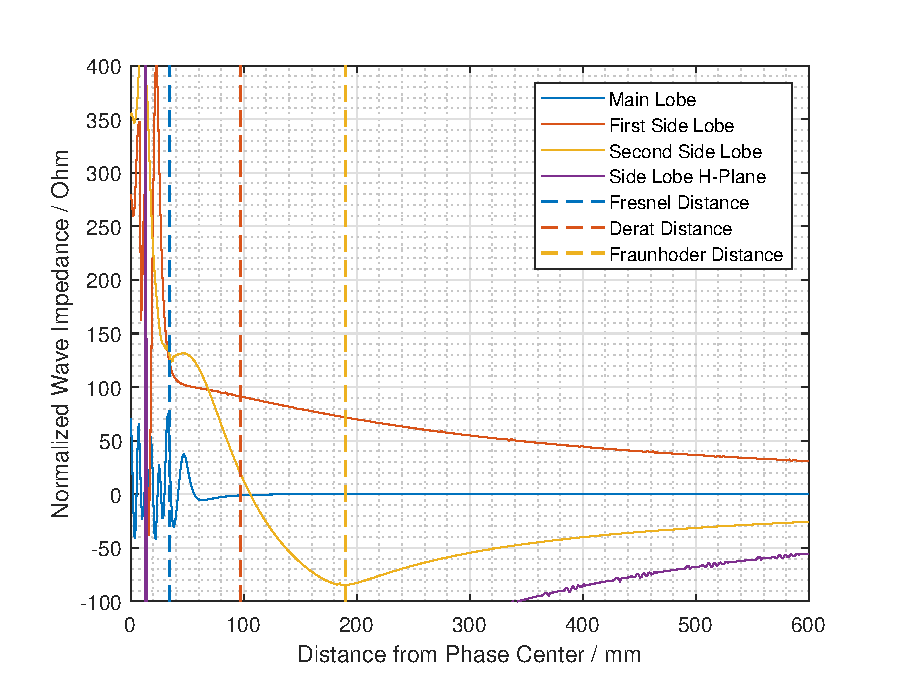
\includegraphics[width=0.49\textwidth]{Matlab/NormWaveImpHorn.eps}}
  \centering
  \subfigure[Phase]{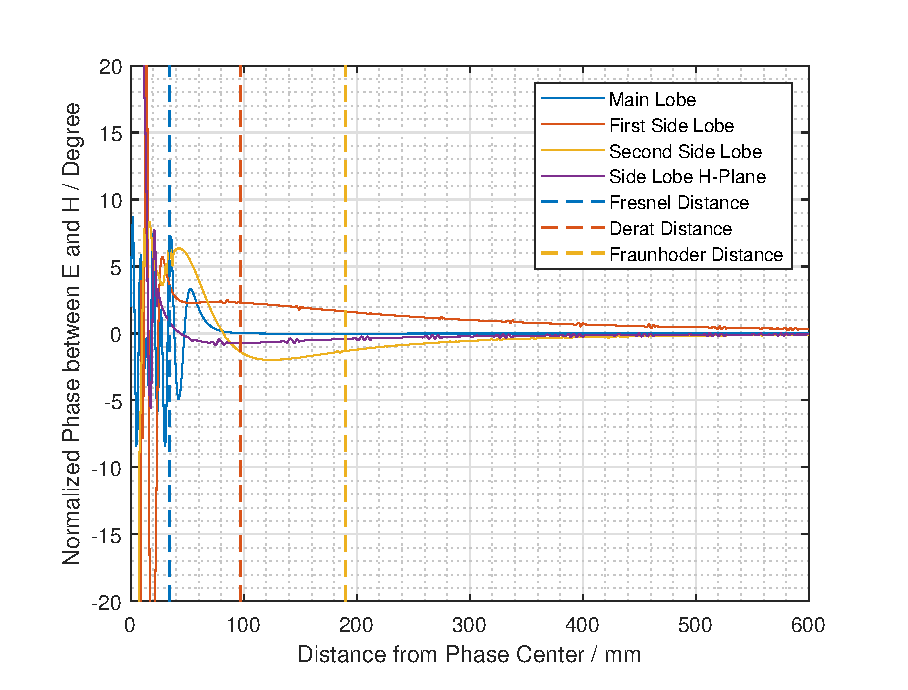
\includegraphics[width=0.49\textwidth]{Matlab/NormPhaseHorn.eps}}
  \centering
  \subfigure[EIRP]{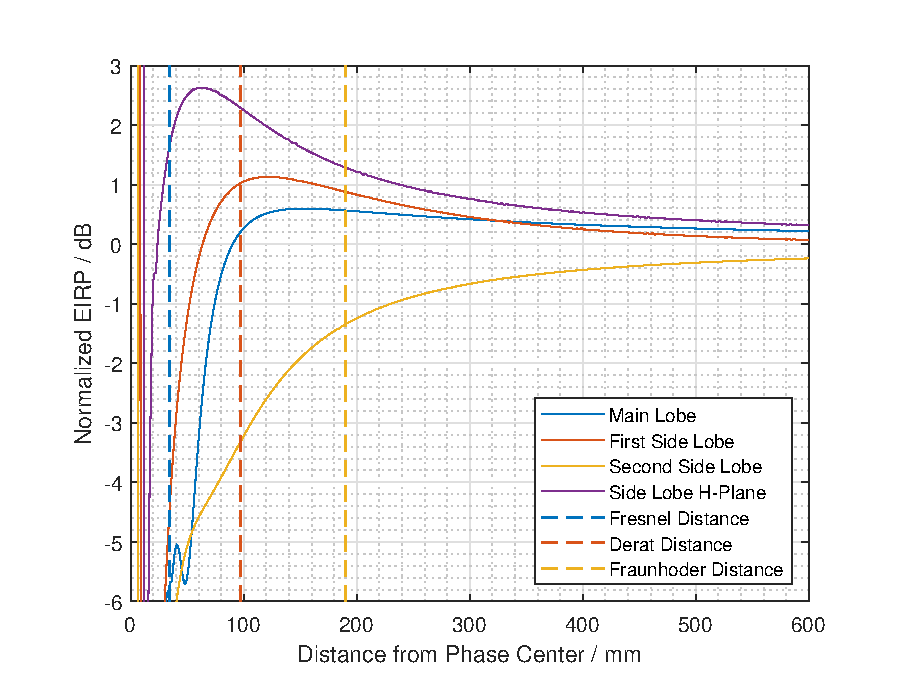
\includegraphics[width=0.49\textwidth]{Matlab/NormEIRPHorn.eps}}
  \centering
  \subfigure[Antenna Pattern E-Plane]{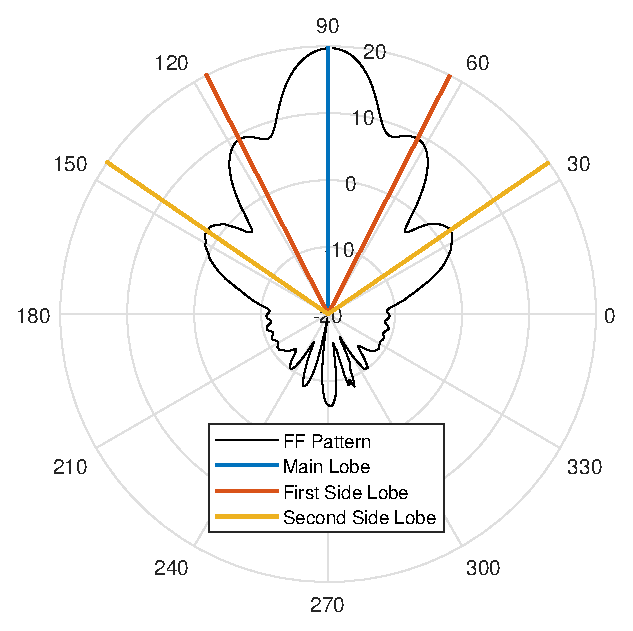
\includegraphics[width=0.35\textwidth]{Matlab/ePlanePattern.eps}}
\caption{Beam comparison of a $\SI{20}{\decibel}$ SGH at $\SI{28}{\giga\hertz}$}
\label{fig:beamcpmp}
\end{figure}

To clarify the introduced distances they will be proved based on a $\SI{20}{\decibel}$ \ac{SGH} at $\SI{28}{\giga\hertz}$. The front view of this horn with the underlying field distribution is plotted in figure \ref{fig:fielddist} in the annex. The polarisation is in $y$-direction, so the $yz$-plane is called E-plane and the $xz$-plane is called H-plane from here on.\\
In figure \ref{fig:beamcpmp} the normalized wave impedance (a), the normalized phase between E- and H-field components (b) and the normalized \ac{EIRP} (c) over the distance to the phase center are plotted. To clarify the designations the directions are plotted in (d). The data have been generated by CST\texttrademark , a full wave simulation tool. Complex data in $x$, $y$, and $z$ direction was exported and post processed to Matlab\texttrademark{}.\\
Also the field boundaries from the sections above are plotted with dashed lines. For the derivation of the field boundaries only the opening of the horn in the E-plane was taken to account. This is sensible because the field distribution and thus the usage of the aperture is known, refer to figure \ref{fig:fielddist}. As it can be seen, in the E-plane the aperture is fully used. But if the field distribution is unknown, the smallest circle enclosing the aperture has to be taken.\\
The main lobe (blue line) is from Derat-distance on in \ac{FF} condition. The wave impedance reached its end value of $120\pi\si{\ohm}\approx\SI{377}{\ohm}$, E- and H-fields are coherent and the \ac{EIRP} value converged. Considering the side lobes it can be seen that in the reactive \ac{NF} the field conditions are very unstable, whereas the fields in the radiating \ac{NF} become more stable. In the \ac{FF} the field values are continually decreasing the offset from their final value.\\
In figure \ref{fig:devantennap} in the annex the resulting antenna patterns in different radii are depicted as well in Cartesian coordinates (a) as in Polar coordinates (b). The assumption 

\begin{equation}
S = \frac{E^2}{Z_0}
\label{eq:poynting}
\end{equation}

was taken to account. In addition analogue to (a) and (b) in (c) the \ac{EIRP} computed in different radii is plotted in figure \ref{fig:fielddist}. At Derat distance ($\approx\SI{100}{\milli\meter}$) the error in main beam direction is about $\SI{0.5}{\decibel}$ and the antenna pattern is further evolving after the Fraunhofer distance at about $\SI{200}{\milli\meter}$.

\section{Spatial Sampling Approaches}

\begin{figure}
\centering
\def\svgwidth{0.4\textwidth}
\input{Bilder/KoordinateSystem.pdf_tex}
\caption{The underlying coordinate system}
\label{coordinates}
\end{figure}

In figure \ref{coordinates} the used coordinate system is depicted. In comparison with a globe the latitude is described by the elevation with the symbol $\Theta$ and the longitude is described by the azimuth with the symbol $\Phi$. The value range of $\Theta$ and $\Phi$ is:

\begin{equation}
-\frac{\pi}{2} \leq \Theta <\frac{\pi}{2}\, ,\quad -\pi \leq \Phi < \pi
\end{equation}

Hereinafter different spatial sampling approaches for this sphere are introduced. For the development of a sampling grid a sampling frequency is necessary and will be introduced in the next section.

\subsection{Derivation of the Spatial Sampling considering the Array Factor}
\label{sec:spasa}

The \ac{AF} is \glqq the radiation pattern of an array antenna when each array element is considered to radiate isotropically\grqq{} \cite{ieeeantenna}. The sampling frequency in either elevation or in azimuth is dependent on the aperture of the \ac{DUT} and the wavelength. To investigate the necessary sampling frequency an one dimensional $\sfrac{\lambda}{2}$ array of isotropic radiators was taken in account. With the number of elements $N$, the element spacing $d = \sfrac{\lambda}{2}$ and the wavelength $\lambda$ the antenna pattern is derivable: \cite{litze}

\begin{equation}
\begin{vmatrix}\Gamma\left(\theta\right)\end{vmatrix}^2 = \Biggl|\frac{\sin\left(\frac{\pi M d}{\lambda \sin\left(\theta\right)}\right)}{\sin\left(\frac{\pi d}{\lambda \sin\left(\theta\right)}\right)}\Biggl|^2 = \Biggl|\frac{\sin\left(\frac{\pi M}{2 \sin\left(\theta\right)}\right)}{\sin\left(\frac{\pi}{2 \sin\left(\theta\right)}\right)}\Biggl|^2
\end{equation}

\begin{figure}[h]
  \centering
  \subfigure[Two elements: Pattern]{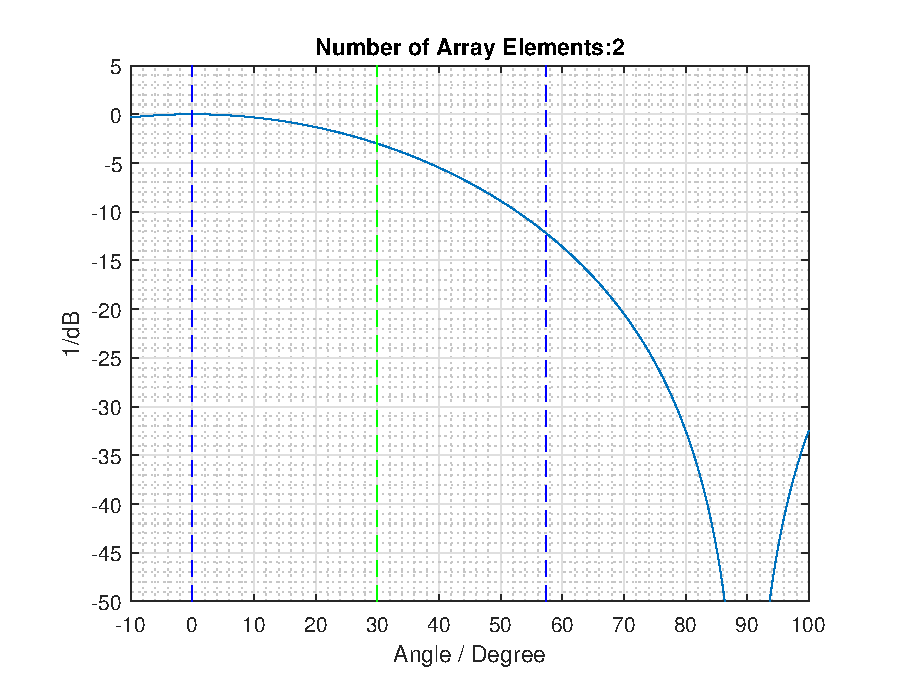
\includegraphics[width=0.32\textwidth]{Matlab/NoNumEl2.eps}}
  \centering
  \subfigure[Six elements: Pattern]{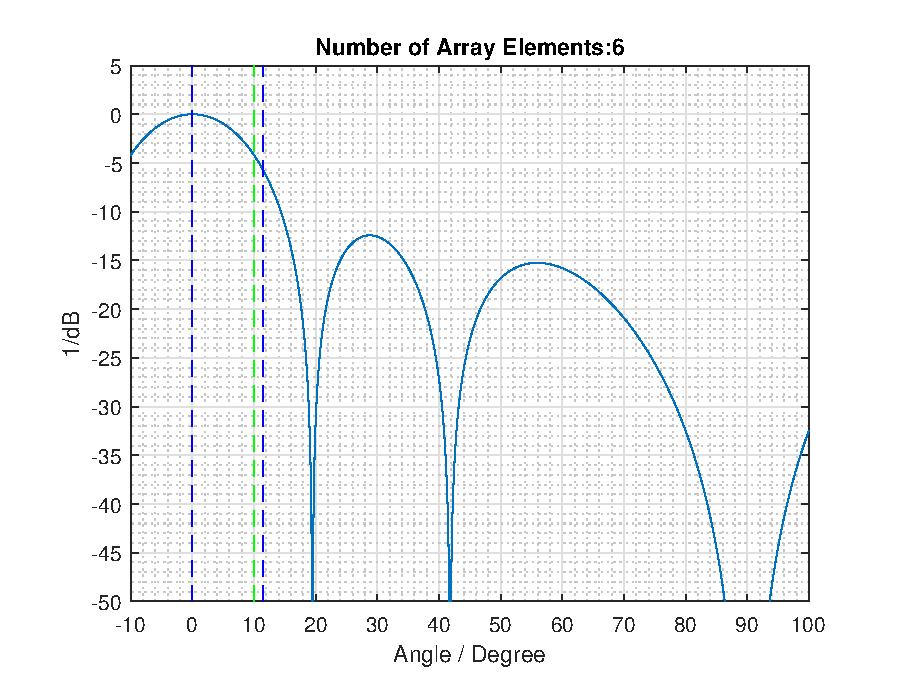
\includegraphics[width=0.32\textwidth]{Matlab/NoNumEl6.eps}}
  \centering
  \subfigure[100 elements: Pattern]{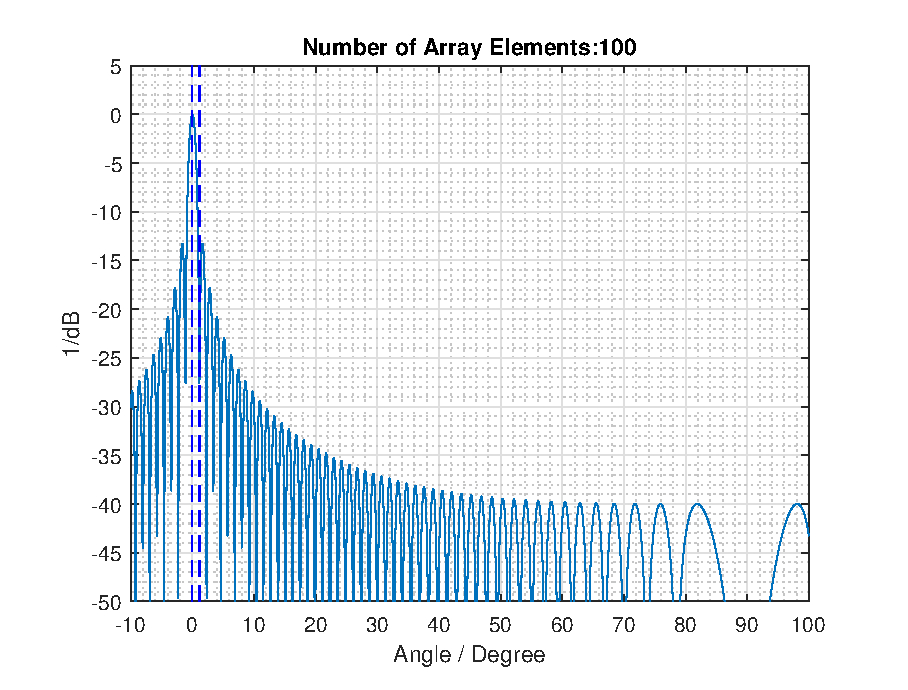
\includegraphics[width=0.32\textwidth]{Matlab/NoNumEl100.eps}}
\caption{Pattern of $N$-element array with $\sfrac{\lambda}{2}$-spacing}
\label{fig:evolvpattern2}
\end{figure}

\begin{figure}[h]
  \centering
  \subfigure[Two elements: Mode spectra]{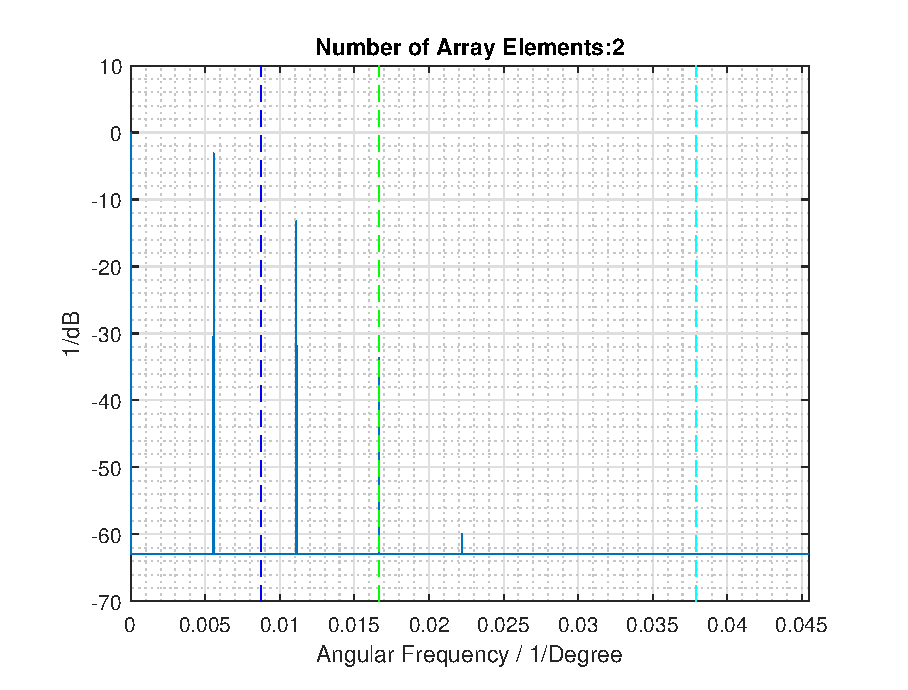
\includegraphics[width=0.32\textwidth]{Matlab/SpNumEl2.eps}}
  \centering
  \subfigure[Six elements: Mode spectra]{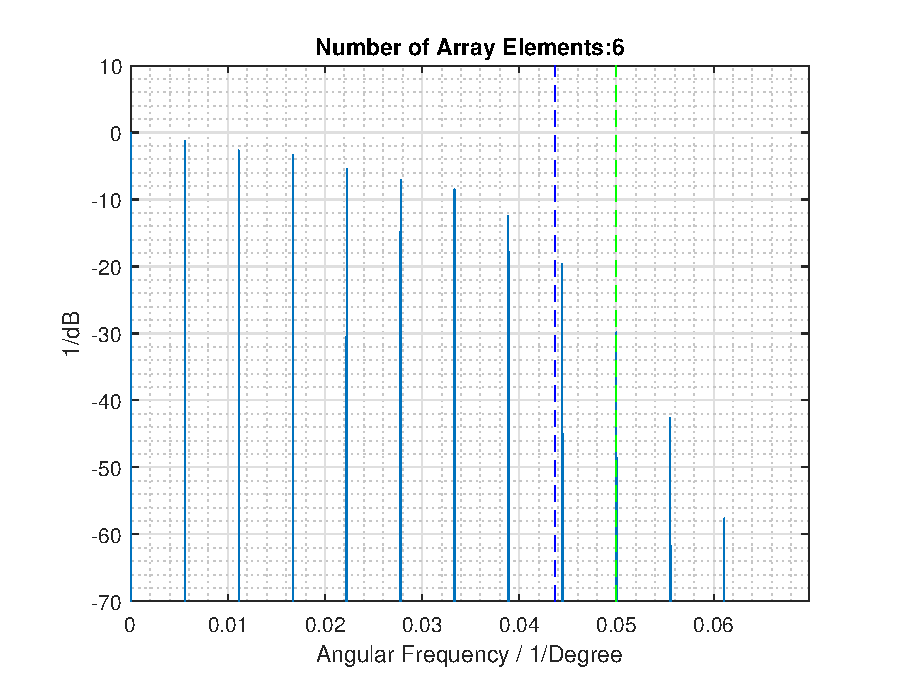
\includegraphics[width=0.32\textwidth]{Matlab/SpNumEl6.eps}}
  \centering
  \subfigure[100 elements: Mode spectra]{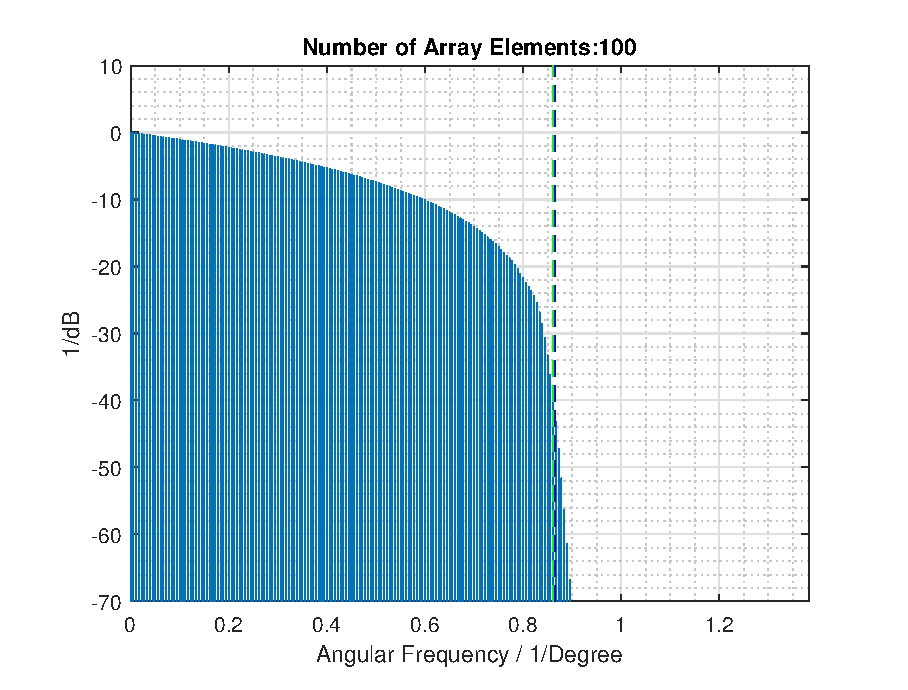
\includegraphics[width=0.32\textwidth]{Matlab/SpNumEl100.eps}}
\caption{Mode spectra of $N$-element array with $\sfrac{\lambda}{2}$-spacing}
\label{fig:evolvpattern3}
\end{figure}

The resulting pattern is depicted in figure \ref{fig:evolvpattern2} and in annex \ref{fig:evolvpattern} (a little larger).\\
In \cite{hansen} it is suggested to use the sampling increment of:

\begin{equation}
\Delta\Theta_\text{Hansen} = \frac{2\pi}{2N+1}\ , \quad \Delta\Phi_\text{Hansen}=\frac{2\pi}{2M+1}
\label{eq:refahansen}
\end{equation}

Where $N$ is the highest significant wave mode on the minimum sphere enclosing the antennas aperture and $M$ is the highest significant wave mode on the minimum cylinder. With the sphere radius $r_S$, the cylinder radius $r_C$ and the angular wavenumber $k = \sfrac{2\pi}{\lambda}$ they are calculated as follows:

\begin{equation}
N = kr_S+10\ , \quad M = kr_C+10
\end{equation}

For example, the resulting formula for the reference angle increment in elevation is calculated in \cite{2018arXiv180310993F} as

\begin{equation}
\Delta\Theta_{\text{ref}} = \lim_{r_S \to \infty}\Delta\Theta' = \lim_{r_S \to \infty} \frac{2\pi}{2\left(kr_S+10\right)+1} = \frac{\lambda}{2\cdot r_S},
\label{eq:hansenrefa}
\end{equation}

the reference angle increment in azimuth as

\begin{equation}
\Delta\Phi_{\text{ref}} = \frac{\lambda}{2\cdot r_C}.
\end{equation}

To illustrate these angle increments the one dimensional array of isotropic radiators is taken. Evaluating the \ac{AF} of a $d = \sfrac{\lambda}{n}$ -array with $N$ elements the reference angle becomes very short:

\begin{equation}
\Delta\Phi_{\text{ref}} = \frac{n}{N-1}
\label{eq:1dinc}
\end{equation}

With the \ac{FFT} over the angle of the antenna patterns from figure \ref{fig:evolvpattern2} the mode spectra can be derived and is seen in figure \ref{fig:evolvpattern3} (or \ref{fig:evolvpattern} in annex).\\
When an arbitrary signal is sampled, the spectrum is mirrored at the sampling frequency. Choosing a sampling frequency lower than twice the highest occurring frequency in the sampled signal causes an irreversible error. This is called the Nyquist-Shannon sampling theorem.\\
For that sake the dashed lines are:

\begin{equation}
\color{blue}\left(\Delta\Phi_{\text{ref}}\right)^{-1}\color{black},\ \color{cyan}\left(\Delta\Phi_\text{Hansen}\right)^{-1}\color{black}\ \text{and}\ \color{green}\text{first mode} > \SI{-40}{\decibel} \color{black}
\end{equation}

Similar to that the dashed lines in figure \ref{fig:evolvpattern2} are the first sampling points using the derived sampling frequency.\\
The issue is now to find the sampling frequency at which the sampling error is independent from the aperture of the antenna. As depicted in figure \ref{fig:evolvpattern3} the sampling frequency introduced by \cite{hansen} is to strict for small apertures. On the other hand the reference angle introduced by \cite{2018arXiv180310993F} is to inaccurate for small apertures. Because of that the new \ac{CrefA} is taken:

\begin{equation}
\text{CrefA} = \left(\Delta\Phi_{\text{ref}}\cdot\left(\text{first mode} > \SI{-40}{\decibel}\right)\right)^{-1}
\end{equation} 

\begin{figure}
\centering
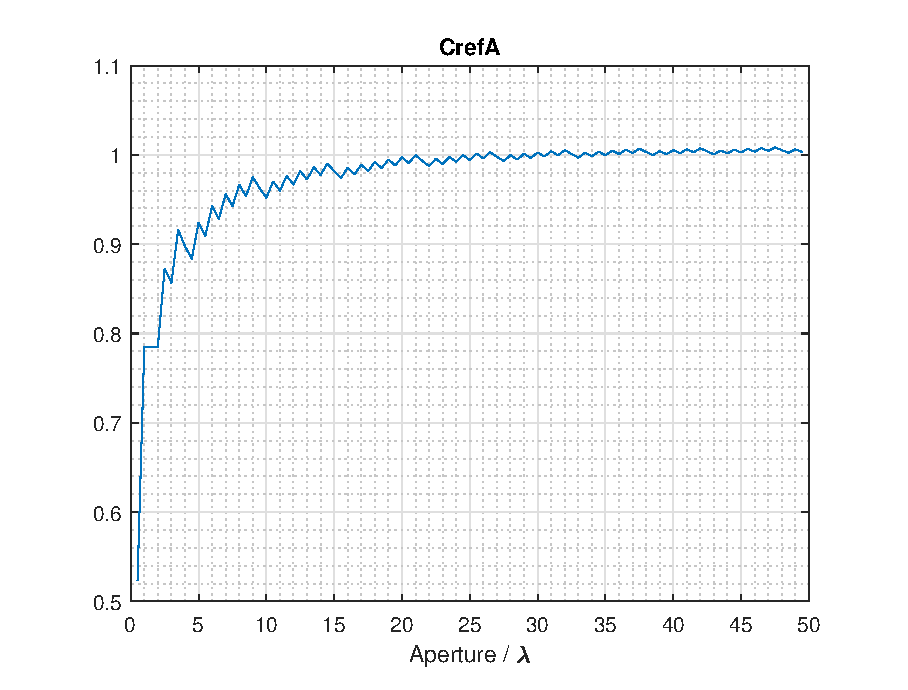
\includegraphics[width=0.41\textwidth]{Matlab/CrefA.eps}
\caption{Correction Factor Reference Angle}
\label{fig:crefa}
\end{figure}

This factor is plotted in figure \ref{fig:crefa}. It is dependent of the aperture. With that the error due to sampling is independent from the antennas aperture. Less than $\SI{-40}{\decibel}$ in the mode spectra is defined for the reference angle increment in \cite{2018arXiv180310993F}, compare figure \ref{fig:evolvpattern3}.\\
For further reduction of points a second factor is introduced, the \acf{SF}. At $\text{SF}=2$ every second measurement point is skipped. With all that the angle increments for spherical sampling is:

\begin{equation}
\Delta\Theta = \text{SF}\cdot\text{CrefA}\left(\sfrac{2r_S}{\lambda}\right)\cdot\frac{\lambda}{2r_S}\ ,\quad\Delta\Phi = \text{SF}\cdot\text{CrefA}\left(\sfrac{2r_C}{\lambda}\right)\cdot\frac{\lambda}{2r_C}
\label{eq:angle}
\end{equation}

\subsection{Constant Step Size Grid}


\begin{figure}[h]
  \centering
  \subfigure[$\text{CTF}=0$; spherical presentation]{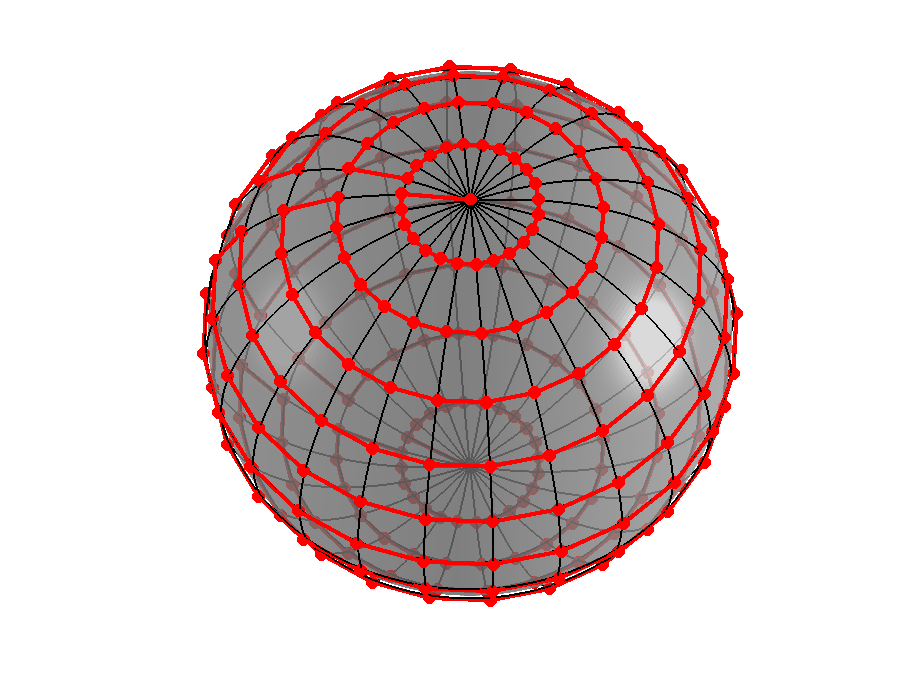
\includegraphics[width=0.49\textwidth]{Matlab/GridCoStPolar.eps}}
  \centering
  \subfigure[$\text{CTF}=1$; spherical presentation]{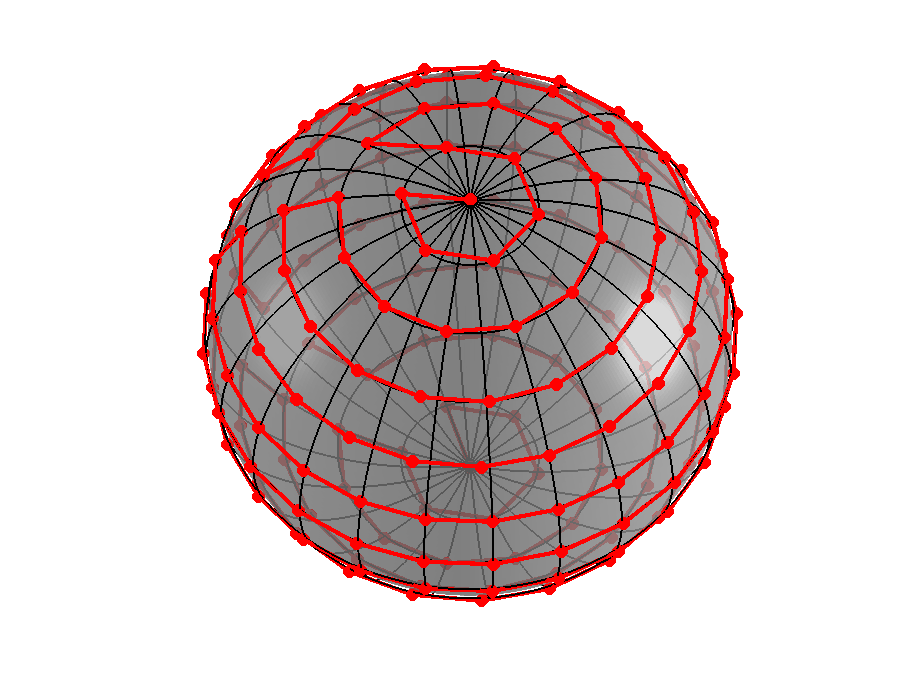
\includegraphics[width=0.49\textwidth]{Matlab/GridCoStSinPolar.eps}}
  \centering
  \subfigure[$\text{CTF}=0$; Cartesian presentation]{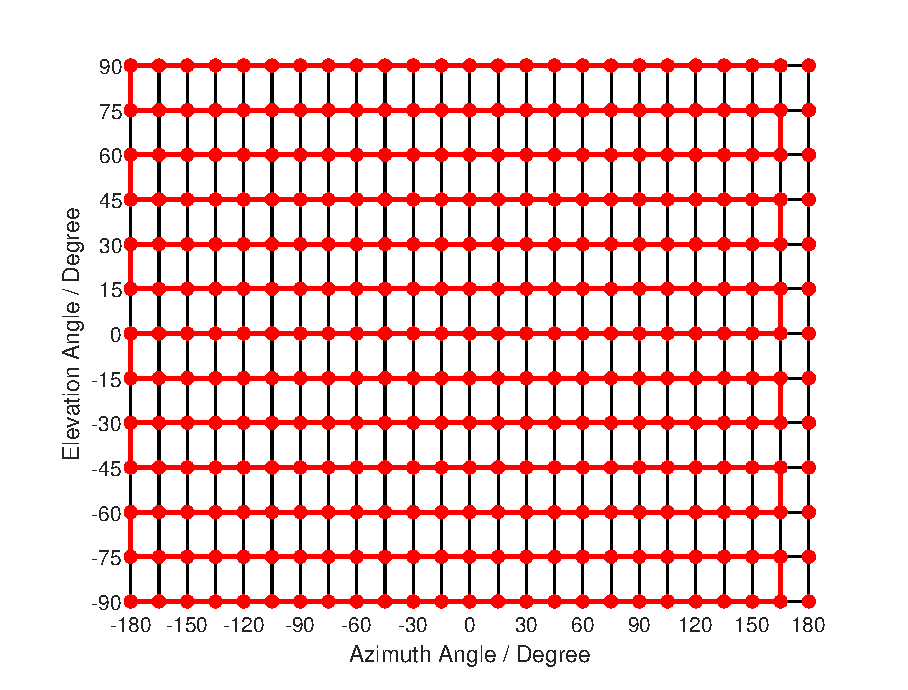
\includegraphics[width=0.49\textwidth]{Matlab/GridCoStCart.eps}}
  \centering
  \subfigure[$\text{CTF}=1$; Cartesian presentation]{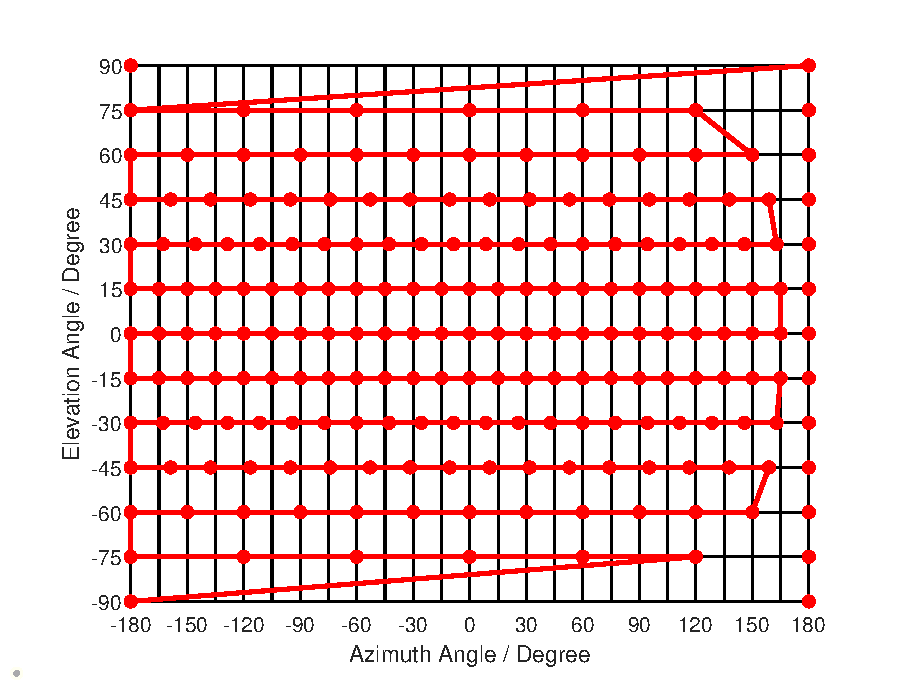
\includegraphics[width=0.49\textwidth]{Matlab/GridCoStSinCart.eps}}
\caption{$\SI{15}{\degree}$ -Constant Step Size Grid}
\label{fig:cssg}
\end{figure}

The most straight forward way to a spherical measurement is using a \ac{CSSG} depicted in figure \ref{fig:cssg} (a). The advantage is the easy feasibility with any positioner. This is visual in \ref{fig:cssg} (c), where the angles are printed in Cartesian coordinates. Ether the azimuth can be swept on every latitude circle or the elevation can be swept on every longitude circle. On the other hand the measurement density is higher on the poles than on the equator.\\
To meet that the theta dependent number of azimuth points was introduced e.g. by \cite{ctiaat}. It is applied as follows:

\begin{align}
N_{\text{max}} = \frac{2\pi}{\Delta\Phi}\\
N\left(\Theta\right)=\lceil N_{\text{max}}\cdot\cos\left(\Theta\right)\rceil\\
\Delta\Phi\left(\Theta\right) = \frac{2\pi}{N\left(\Theta\right)}
\end{align}

It is only possible to sweep the azimuth when this type of grid is used. Here also the Cartesian coordinates are plotted in (d). The red line is a suggested sequence.

\subsection{Constant Density}

\begin{figure}[h]
  \centering
  \subfigure[Polar Coordinates]{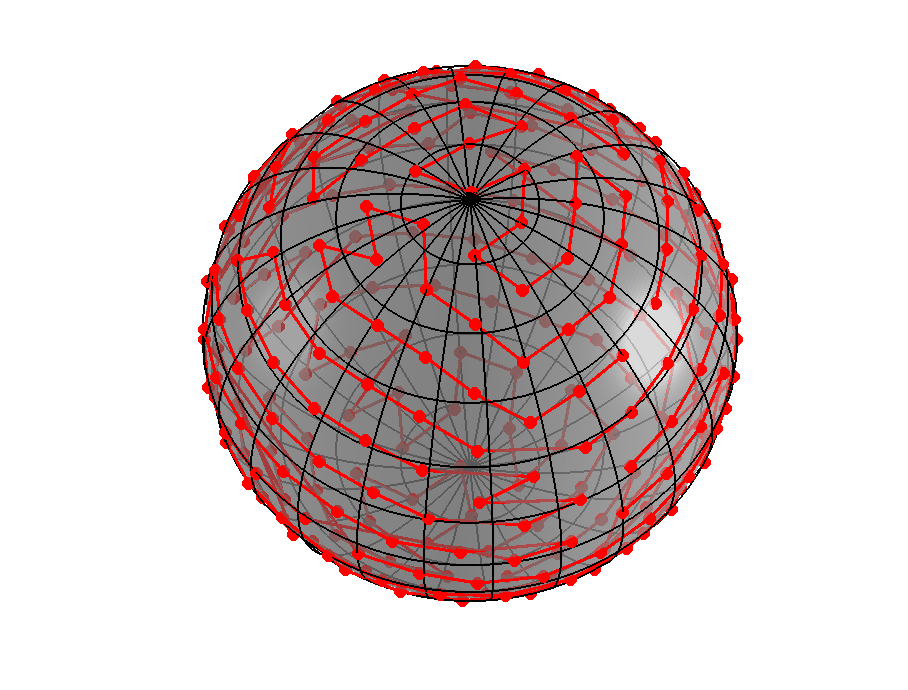
\includegraphics[width=0.49\textwidth]{Matlab/GridCoDePolar.eps}}
  \centering
  \subfigure[Cartesian Coordinates]{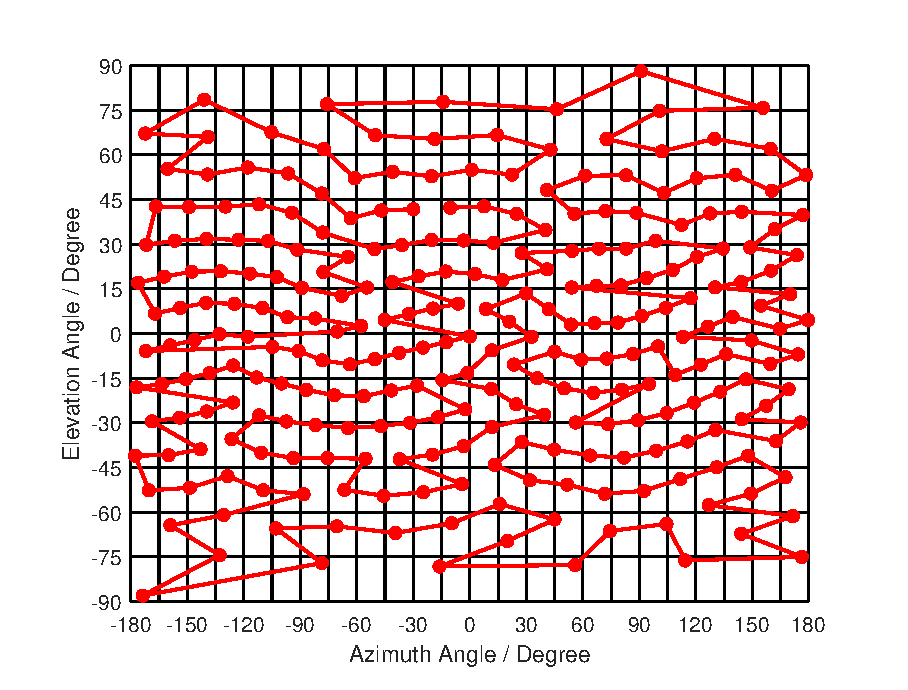
\includegraphics[width=0.49\textwidth]{Matlab/GridCoDeCart.eps}}
\caption{Constant Density Grid with 264 Measurement points}
\label{fig:cdg}
\end{figure}

The \ac{CDG} depicted in figure \ref{fig:cdg} was produces and generated by a charged particle algorithm. It works by minimising the cumulated potential energy of all measurement dots considered as charged particles. The potential energy is minimal, when all points are evenly distributed over the sphere.\\ 
Deriving the optimal measurement sequence is a \ac{TSP}. It is solved by the Matlab toolbox introduced in \cite{tsp} viewing the angles as Cartesian coordinates. This path is optimized for the positioner to move as efficient as possible. Because the positioning in Azimuth is faster than in Elevation, the elevation distance is weighted five times more. Furthermore the periodicity is taken to account, so that the distance between tow points $\text{P}_n$ and $\text{P}_m$ is:

\begin{equation}
\Delta\Theta_{mn} = 5\left(\Theta_{\text{P}_n}-\Theta_{\text{P}_m}\right)\ ,\quad \Delta\Phi_{mn} = \text{min}\left(|\Phi_{\text{P}_n}-\Phi_{\text{P}_m}|\, ,\ 2\pi-|\Phi_{\text{P}_n}-\Phi_{\text{P}_m}|\right)
\end{equation}

With that the quadratic distance Matrix $D$ can be derived using euclidean distance with $d_{mn} = \sqrt{\Delta\Theta_{mn}^2+\Delta\Phi_{mn}^2}$ out of $N$ Points:

\begin{equation}
D = \begin{bmatrix}
 0 & d_{12} & \dots & d_{1N}\\
 d_{21} & 0 & \dots & d_{2N}\\
 \vdots & \vdots & \ddots & \vdots\\
 d_{N1} & d_{N2} & \dots & 0
\end{bmatrix}
\end{equation}

The cumulated distance for $N = 264$ is converged after around one million iterations. The result is depicted in figure \ref{fig:cdg} (b).

\subsection{Other}

There are other grid types, which are mainly based on the already introduced grids. First there are Cardinal cuts, here a measurement is carried out along the equator and one, tow or more orthogonal meridians. If the alignment is right a technique called \acf{PM} can be used to calculate the complete antenna pattern out of the cardinal cuts. The problem here is that a symmetry is assumed which is always wrong if the direction of main beam and the orientation of the pattern is unknown. \cite{2018arXiv180310993F}\\
An other spatial sampling approach is the Spiral Scan. It is developed by \ac{RS} and can be used for a pre scan to find the maximum \ac{EIRP} direction. Here elevation and azimuth is swept. \cite{ctiaat}

\section{Total Radiated Power Quadratures}
\label{sec:quadrature}

The easiest way to derive the \ac{TRP} is if Cardinal cuts or a \ac{CDG} was taken, to compute the mean of all \ac{EIRP} samples. For other grids the quadrature needs to be done as follows. \cite{trp}

\subsection{Sine Theta}

The straight forward way is to transform the integral over a spherical surface $S$

\begin{equation}
\text{TRP} = \frac{1}{4\pi}  \oiint_S \text{EIRP}\left(\theta,\phi\right)\cdot\sin\theta\cdot d\theta d\phi
\label{eq:trpint}
\end{equation}

to a sum, this is called quadrature. The easiest approach is carried out by discretizing the integral Argument:  \cite{ctiaat}

\begin{equation}
\frac{1}{4\pi}\cdot\sin\theta\cdot d\theta\cdot d\phi \ \Rightarrow\ \frac{1}{4\pi}\cdot \Delta\theta\cdot \Delta\phi\cdot\sin\theta = \frac{1}{4\pi}\cdot \frac{\pi}{N}\cdot \frac{2\pi}{M}\cdot\sin\theta=\frac{\pi}{2NM}\cdot\sin\theta
\end{equation}

With that the quadrature is:

\begin{equation}
\text{TRP}_{\sin\theta} = \frac{\pi}{2NM}\sum^{N-1}_{i=1}\sum^{M-1}_{j=0}\left(\text{EIRP}_\theta\left(\theta_i,\phi_j\right)+\text{EIRP}_\phi\left(\theta_i,\phi_j\right)\right)\cdot\sin\left(\theta_i\right)
\label{eq:trpsumsin}
\end{equation}

$N$ is the number of angular intervals in $\theta=\left[0,\pi\right[$ (elevation), $M$ is the number of angular intervals in $\phi=\left[0,2\pi\right[$ (azimuth), the indices $i=\left[0,N\right]$, $j=\left[0,M\right]$ and the \ac{EIRP} is split in its horizontal ($\text{EIRP}_\phi$) and its vertical ($\text{EIRP}_\theta$) part. This quadrature is called sine theta.

\subsection{Clenshaw-Curtis}

Because the sine theta quadrature is not accurate for spars measurements and the measurement points at the poles are neglected, an other weighting scheme is used, the \ac{CC}-quadrature. For the sine theta quadrature the integrating surface is constantly interpolated (compare equation \ref{eq:trpsumsin}). The \ac{CC} quadrature is more accurate using the weights W computed by expending the integrand with Chebyshev polynomials. With that formula \ref{eq:trpsumsin} develops to: \cite{trp}

\begin{equation}
\text{TRP}_{\text{CC}} = \frac{1}{2M}\sum^{N-1}_{i=1}\sum^{M-1}_{j=0}\left(\text{EIRP}_\theta\left(\theta_i,\phi_j\right)+\text{EIRP}_\phi\left(\theta_i,\phi_j\right)\right)\cdot\text{W}\left(\theta_i\right)
\label{eq:trpsumcc}
\end{equation}

\subsection{Jacobi}

The Jacobi quadrature uses the area of triangles on the spherical surface between the measurement points. The average \ac{EIRP} of a triangle is computed and weighted by the area $A_i$ of it. The result is normed with the complete surface area. With that for every triangle $i=\left[1,N\right]$ the \ac{TRP} quadrature is: \cite{trp}

\begin{equation}
\text{TRP}_{\text{J}} = \frac{\sum^N_{i=1}A_i\left(\frac{\text{EIRP}_{0,i}+\text{EIRP}_{1,i}+\text{EIRP}_{2,i}}{3}\right)}{\sum^N_{i=1}A_i}
\end{equation}

\subsection{Comparing the Quadratures}

Sine Theta- and \ac{CC} quadratures are only applicable for \acp{CDG} and with slight optimizations also for \acp{CDG} with less dense measurements at the poles. Whereas the Jacobi quadrature can be used for arbitrary grids.\\
In \cite{trp2} it is investigated which quadrature leads to the most accurate result with the same number of points. The result is that \ac{CC}- and Jacobi quadratures are equally accurate.

\section{Statistics and Regression}

This section shall give a brief introduction in the field of statistics and regression, which is necessary for the spatial sampling simulation. First statistical terms, than methods to display scatterings and multidimensional regressions are introduced.

\subsection{Metrics to Describe Distributions}

To describe a one dimensional scattering $h$ with $N$ samples $x$ and the cumulative frequency $H$, these terms are regularly used: \cite{dffs}

\begin{itemize}
\item The commonly most used and known term is the \textbf{Arithmetic Mean}, which is vulnerable by outliers and computed as:
\begin{equation}
\bar x = \frac{1}{N}\sum_{n=1}^N x_N
\end{equation}
\item The \textbf{Median} is that value lying in the middle of a distribution, so that $H\left( x\right) = 0.5$. It is computed by sorting the samples by value and, if the number of samples is even, taking the mean of the two samples in the middle, or if the number of samples is odd taking the middle value.
\item The \textbf{Variance} of a distribution is the sum of squared error, normalized by the number of samples. This metric is strongly vulnerable by outliers. The computation is as follows:
\begin{equation}
s^2 = \frac{1}{N-1}\sum_{n=1}^N\left( x_n-\bar{x}\right)^2
\end{equation}
\item The \textbf{$p$-Quantile} is analogue to the Median, that value of a sorted sample vector where $P$ percent of the distributions values is reached, hence $H\left( x\right) = p$.
\item A more stable metric for scattering as the variance is the \textbf{\ac{IQR}}, this describes the range between two quantiles.
\end{itemize}

\subsection{Display a Distribution}

The commonly known way to display a distribution is a bar diagram. There the value of range is split in $M$ bars displaying the values in the $x$-axis and the probability of each bucket on the $y$-axis. An other way to display a distribution is the box-plot, where only the minimal, maximal, $\SI{25}{\percent}$-quantile, median and $\SI{75}{\percent}$-quantile value is plotted.

\subsection{Distribution Functions}
There are all sorts of scattering distributions e.q. even distribution, Weibull distribution, Rayleigh distribution, ... but the most prominent distribution is the normal distribution by Gauss:

\begin{equation}
f\left( x \right) = \frac{1}{\sigma\sqrt{2\pi}}e^{-\frac{1}{2}\left(\frac{x-\mu}{\sigma}\right)^2}
\end{equation}

Assuming that $\sigma = s$ and $\mu = \bar{x}$ this function can also be plotted and used for predictions.

\subsection{Regression of multidimensional Datasets}
\label{sec:regod} 
Assuming a input variable vector $\vec{x}$, a coefficient set $\vec{b}$ and a result $y$ an arbitrary polynomial can be written as: \cite{sip}

\begin{equation}
y\left(\vec{x}\right) = \vec{x}^{\mathsf T}\cdot\vec{b}=\begin{bmatrix}
1 & x_1 & x_2 & \dots & x_M
\end{bmatrix} \cdot \begin{bmatrix}
b_0 \\ b_1 \\ b_2 \\ \vdots \\ b_M
\end{bmatrix}
\end{equation}

The regression is about estimating the coefficient vector $\vec{b}$. With $N$ samples this system is overdetermined which leads to an error vector $\vec{e}$. Than the resulting polynomial is:

\begin{equation}
\vec{y}=X\cdot \vec{b}+\vec{e}=\begin{bmatrix}
y_1 \\ y_2 \\ \vdots \\ y_N
\end{bmatrix} = \begin{bmatrix}
1 & x_{11} & x_{12} & \dots & x_{1M} \\
1 & x_{21} & x_{22} & \dots & x_{2M} \\
\vdots & \vdots & \vdots & \ddots & \vdots \\
1 & x_{N1} & x_{N2} & \dots & x_{NM}
\end{bmatrix} \cdot \begin{bmatrix}
b_0 \\ b_1 \\ b_2 \\ \vdots \\ b_M
\end{bmatrix} + \begin{bmatrix}
e_1 \\ e_2 \\ \vdots \\ e_N
\end{bmatrix}
\end{equation}

The sum square error

\begin{equation}
S = \vec{e}^{\mathsf T}\cdot\vec{e}=\left(\vec{y}-X\cdot\vec{b}\right)^{\mathsf T}\cdot\left(\vec{y}-X\cdot\vec{b}\right)
\end{equation}

is minimized by 

\begin{equation}
\nabla_{\vec{b}}\cdot S = 0
\end{equation}

leading to the well known \ac{LS}-method

\begin{equation}
\hat{b}_\text{LS}=\left(X^{\mathsf T} X\right)^{-1} X^{\mathsf T}\vec{y}.
\end{equation}

The input matrix $X$ can also be optimized by taking combinations or powers of different dependent parameters.\\
A frequent problem is that the significance of the parameters in $\vec{b}$ is unknown, hence to unnecessary high number of parameters and inaccurate regressions. Therefore the hypothesis that $b_m=0$ is checked. The parameters in vector $\vec{b}$ are t-distributed. First the covariance matrix of the independent variable $\vec{y}$ is estimated: \cite{dffs}

\begin{equation}
C = \left(X^{\mathsf T} X\right)^{-1}\frac{1}{N-M-1}\cdot\left(\vec{y}^{\mathsf T}\cdot\vec{y}-\vec{b}^{\mathsf T}\cdot X^{\mathsf T}\cdot \vec{y}\right) = \begin{bmatrix}
c_{00} & c_{01} & \dots & c_{0M} \\
c_{10} & c_{11} & \dots & c_{1M} \\
\vdots & \vdots & \ddots & \vdots \\
c_{M0} & c_{M1} & \dots & c_{MM}  
\end{bmatrix}
\end{equation}

With the variances $c_{mm}$ of each parameter and the variance of $\vec{y}$ $s$, the $p$-value can be computed with $F_t$, the \ac{CDF} of the t-distribution with $N-1$ degrees of freedom:

\begin{equation}
p_m = F_t\left(\frac{b_m}{c_{mm}\cdot s}\right)
\end{equation}

Normally a significance value of $\alpha = \SI{5}{\percent}$ is chosen. If the $p$-value is inside the interval $p_m=\left[\sfrac{\alpha}{2},\ 1-\sfrac{\alpha}{2}\right]$ the hypothesis is valid and parameter $m$ can be discarded.

To estimate the confidence interval for the mean of a regression at a point $x_0$ the variance at dot $x_0$ must be computed: \cite{dffs}

\begin{equation}
s_{\hat{y}_0}^2 = \frac{1}{N-M-1}\cdot\left(\vec{y}^{\mathsf T}\cdot\vec{y}-\vec{b}^{\mathsf T}\cdot X^{\mathsf T}\cdot \vec{y}\right)\cdot \vec{x}_0^{\mathsf T}\cdot \left(X^{\mathsf T} X\right)^{-1} \cdot \vec{x}_0
\end{equation}

Choosing a confidence value $\gamma = \SI{95}{\percent}$, the two parameters $k_1$ and $k_2$ can be derived with the inverse \ac{CDF} $F_t^{-1}$ with $N-M-1$ degrees of freedom:

\begin{equation}
k_1 = F^{-1}\left(\frac{1-\gamma}{2}\right),\ k_2 = F^{-1}\left(\frac{1+\gamma}{2}\right)
\end{equation}

And the confidence interval is:

\begin{equation}
\mu_y\left(\vec{x}_0\right) =\left[ y\left(\vec{x}_0\right)-k_2\cdot s_{\hat{y}_0},\ y\left(\vec{x}_0\right)-k_1\cdot s_{\hat{y}_0}\right]
\label{eq:conv}
\end{equation}



\chapter{OTA Basics}

\section{Probe}

\subsection{mm Trumpet}

\subsection{Standard Gain Horn}

\subsection{Open Ended Wave Guide}

\section{Chamber}

\section{Link Budget}

\section{Alignment of the Equipment under Test (Quiet Zone)}

\subsection{Error due to Probe}

\subsection{Error due to Free Space Loss}

\section{Measurement}

\subsection{Detector Settings and their Influence}

\subsection{Resolution Bandwidth vs. Measurement Time}

\cite{funsspec}


\chapter{Statistical Simulation for Spatial Sampling}

The angle increment was derived in section \ref{sec:spasa} and is presented in equation \ref{eq:angle}. To find a compromise between measurement speed and accuracy a perfect trade off in terms of aliasing error has to be found. For a perfect adjustment of the measurement uncertainty dependent of the \ac{SF} the measurement error shall be independent from the devices aperture.

\section{Implementation}

The simulation is similar to section \ref{sec:spasa}, carried out using the \ac{AF}, however with a two dimensional rectangular $\sfrac{\lambda}{2}$-element spacing array. This brings the advantage that the array size can easily be adjusted. The \ac{FF}-pattern is computed with the Matlab\texttrademark{} class \textit{phased.URA}. Here also a steering vector, consistent of an azimuth and an elevation angle, to specify which direction the main beam of the array is facing, can be handed. The sampling of the \ac{FF}-pattern is accomplished by the included \textit{pattern(...)} function.\\
This simulation is mainly developed for \acp{CSSG} and the angle increment is computed by equation \ref{eq:angle}. With the number of elements in $z$ direction $N_z$ and the number of elements in $y$ direction $N_y$ the radii $r_s$ and $r_c$ can be computed as

\begin{equation}
2r_s = \sqrt{\left(N_y-1\right)^2+\left(N_z-1\right)^2}\cdot\frac{\lambda}{2},\quad 2r_c=\left(N_y-1\right)\cdot\frac{\lambda}{2},
\end{equation}

resulting in an angle increment of

\begin{equation}
\Delta\Theta^\prime = \frac{\text{SF}\cdot\text{CrefA}\left(\sfrac{2r_s}{\lambda}\right)\cdot 2}{\sqrt{\left(N_y-1\right)^2+\left(N_z-1\right)^2}}\ ,\quad\Delta\Phi^\prime = \frac{\text{SF}\cdot\text{CrefA}\left(\sfrac{2r_c}{\lambda}\right)\cdot 2}{\left(N_y-1\right)}.
\end{equation}

Whereby \ac{CrefA} is a function of diameter in wavelength, compare fig. \ref{fig:crefa}. The number of points on each longitude half circle $N_\Theta$ and on each latitude circle $N_\Phi$ is computed and round up:

\begin{equation}
N_\Theta = \bigg\lceil\frac{\pi}{\Delta\Theta^\prime}\bigg\rceil ; \quad N_\Phi^\prime = \bigg\lceil\frac{2\pi}{\Delta\Phi^\prime}\bigg\rceil
\end{equation}

For more sparse sampling at the poles the \ac{CTF} with a value range of $\text{CTF}=\left[0,1\right]$ is introduced to gain Theta dependent azimuth step size:

\begin{equation}
N_\Phi\left(\Theta\right) = \bigg\lceil\frac{2\pi}{\Delta\Phi^\prime}\left(1-\text{CTF}+\text{CTF}\cdot\cos\right(\Theta\left)\right)\bigg\rceil
\end{equation}

If the \ac{CTF} is independent from the resulting uncertainty, than $\text{CTF}=1$ can be chosen and thereby measurement samples saved. For easier computation $N_\Phi\left(\Theta\right)$ is round to 

\begin{equation}
N_\text{round} = \bigg\lceil \frac{N_\Phi^\prime}{k} \bigg\rceil, \ k \in \mathbb{N}
\end{equation}

and not just to the greater integer. So that the angle increment is

\begin{equation}
\Delta\Theta = \frac{\pi}{N_\Theta} , \quad \Delta\Phi\left(\Theta\right) = \frac{2\pi}{N_\Phi\left(\Theta\right)}.
\end{equation}

With the integers in $N_\text{round}$ the advantage is that a uniform \ac{CSSG} can be sampled and the theta dependent phi can be simulated by discarding every $k$\textsuperscript{th} value in each azimuth circle.

\section{Set Up}

\begin{figure}
  \centering
  \subfigure[PDF]{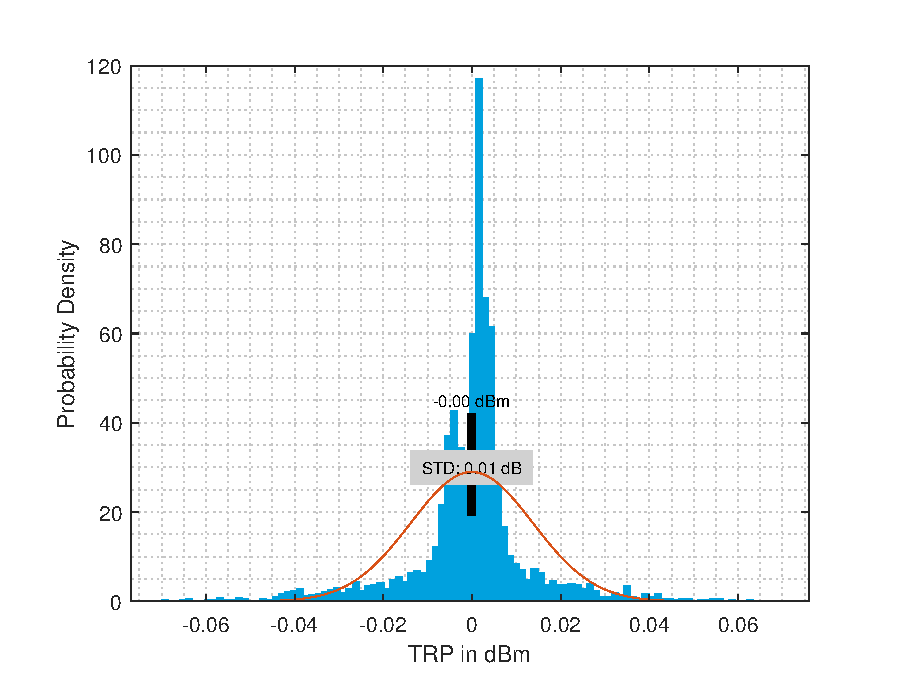
\includegraphics[width=0.49\textwidth]{Matlab/PDF_6-18_SF1.eps}}
  \centering
  \subfigure[CDF]{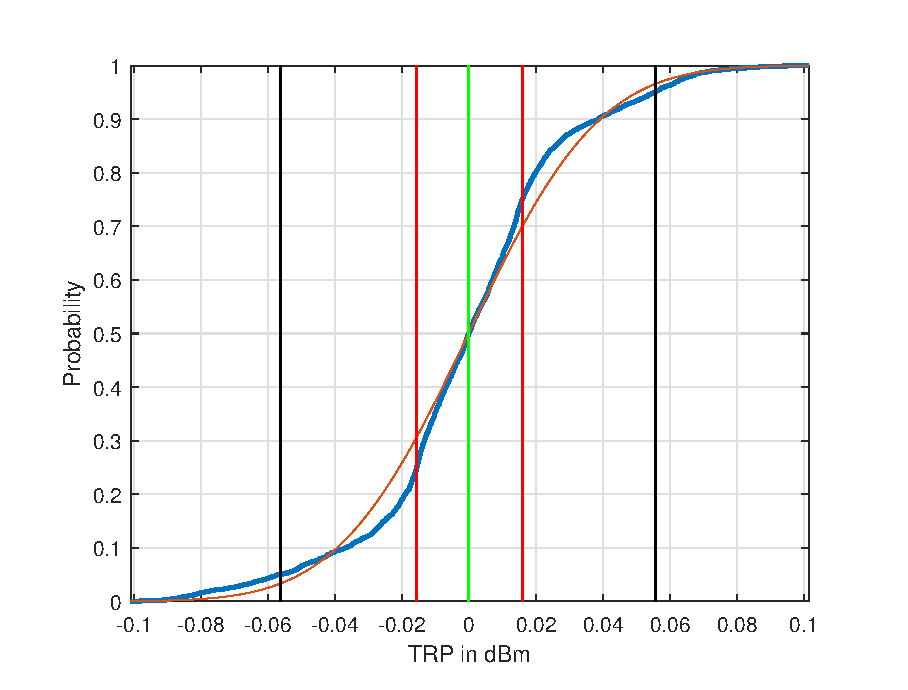
\includegraphics[width=0.49\textwidth]{{Matlab/CDF_6-18_SF1.eps}}}
\caption{4000 random steering vectors, $\text{SF}=1$, 6x18-Array}
\label{fig:rands}
\end{figure}

There are four input parameters: First the \ac{SF}, second the \ac{CTF} and third and fourth the elements of the array in $y$ and $z$ direction. Every set of parameters is simulated with $N=4000$ samples using random steering vectors. The azimuth steering is evenly distributed over the whole circle from $-\pi$ to $\pi$. In elevation a random variable is generated with a \ac{CDF} of \ac{CC} coefficients from $-\sfrac{\pi}{2}$ to $\sfrac{\pi}{2}$ by projecting evenly distributed random numbers. With that the main beam direction is evenly distributed over the spheres surface. For every set of parameters the third step is iterated $N$ times:

\begin{enumerate}
\item Generate $N$ steering vectors.
\item Derive a \ac{CSSG}.
\item Compute the \ac{TRP}:
\begin{enumerate}
\item Generate a antenna pattern using a random steering vector. A sample for that is depicted in fig. \ref{fig:randp}.
\item Sample the antenna pattern with the derived grid.
\item Discard samples dependent on the \ac{CTF}.
\item Compute a \ac{TRP} using the \ac{CC}-quadrature.
\end{enumerate}
\end{enumerate}

A histogram and the resulting \ac{CDF} is plotted in fig. \ref{fig:rands} (a) and (b). In both diagrams additionally the \ac{PDF}, respectively \ac{CDF} of the normal distribution is plotted in orange. Because the normal distribution is not a accurate metric for the underlying distribution, the $\SI{90}{\percent}$ \ac{IQR}, from the $\SI{5}{\percent}$ quantile to the $\SI{95}{\percent}$ quantile, is used to describe the scattering. In fig. \ref{fig:rands} (b) the black lines are the $\SI{5}{\percent}$- and $\SI{95}{\percent}$- quantiles, the red lines the $\SI{25}{\percent}$- and $\SI{75}{\percent}$- quantiles and the mean is the green line.\\
The statistical experimental design is based on a D-optimal design dependent on the parameter matrix

\begin{equation}
X = \begin{bmatrix}
1 & \text{SF}_1 & \text{SF}_1^2 & \text{CTF}_1 & N_{y,1} & N_{z,1} & N_{y,1}N_{z,1}\\
\vdots & \vdots & \vdots & \vdots & \vdots & \vdots & \vdots\\
1 & \text{SF}_N & \text{SF}_N^2 & \text{CTF}_N & N_{y,N} & N_{z,N} & N_{y,N}N_{z,N}
\end{bmatrix}
\label{eq:parammatrix}
\end{equation}

with $M=7$ parameters. The D-optimal design is used because out of other documents e.q. \cite{2018arXiv180310993F} a course assumption to the significant parameters can be derived and thereby not every interaction needs to be tested. It is assumed that the \ac{SF} has also a quadratic dependency and that the linear interactions between the number of elements is significant. With that a minimum number of samples is $N_\text{min}=1.5\cdot\left(M+1\right)=12$ \cite{dffs}. So a statistical experimental design can be derived using the Matlab\texttrademark{} \textit{cordexch(...)}-function with the input of the potency matrix of the regression

\begin{equation}
P = \begin{bmatrix}
0 & 0 & 0 & 0\\
1 & 0 & 0 & 0\\
2 & 0 & 0 & 0\\
0 & 1 & 0 & 0\\
0 & 0 & 1 & 0\\
0 & 0 & 0 & 1\\
0 & 0 & 1 & 1
\end{bmatrix},
\end{equation}

comparing the parameter matrix in equation \ref{eq:parammatrix}. With that the experimental design is derivable as 

\begin{equation}
X^\prime = \begin{bmatrix}
1&1&1&-1&1&-1&-1\\
1&1&1&1&-1&1&-1\\
1&1&1&1&-1&-1&1\\
1&0&0&-1&-1&-1&1\\
1&-1&1&-1&-1&-1&1\\
1&-1&1&-1&1&1&1\\
1&-1&1&1&-1&1&-1\\
1&-1&1&1&-1&-1&1\\
1&1&1&1&1&1&1\\
1&0&0&1&1&1&1\\
1&1&1&-1&1&1&1\\
1&-1&1&-1&-1&1&-1\\
1&0&0&-1&-1&1&-1\\
1&-1&1&1&1&-1&-1\\
1&1&1&-1&1&-1&-1\\
1&0&0&1&1&-1&-1
\end{bmatrix},
\end{equation}

where $1$ stands for the maximum value of the respective variable, analogue $-1$ for minimum and $0$ for middle. To generate a better regression and better possibilities of post processing the experimental design was extended by sweeping every input parameter:

\begin{itemize}
\item The \ac{SF} is swept in the interval $\text{SF}=\left[0.5,1.5\right]$ using $23$ samples.
\item The \ac{CTF} is swept in the interval $\text{CTF}=\left[0,1\right]$ using $3$ samples with equal spacing.
\item The number of $y$ elements is swept in the interval $N_y=\left[2,14\right]$ using $4$ samples.
\item The number of $z$ elements is swept in the interval $N_z=\left[2,22\right]$ using $6$ samples.
\end{itemize}

This results in a experimental design with $N^\prime=23\cdot 3\cdot 4\cdot 6=1656$ samples. The realistic alignment of a array is always that the longer edge in vertical. With that some combinations of array sizes with $N_y > N_z$ are discarded, leading to $N=1380$ combinations. The total number of \ac{TRP} processions and pattern generations is thereby $N_\text{TRP}=1380\cdot 4000 = 5.520.000$. The computation is accomplished by using the parallel \textit{for}-loop by Matlab\texttrademark{} occupying all physical CPUs of a system. Even so the overall duration is in the framework of several days.\\
Furthermore a comparison between \ac{CSSG} and \ac{CDG} shall be accomplished. Therefore the \ac{SF} needs to be projected on a \ac{CDG}. This is accomplished by computing the number of sampling points on the measurement sphere at $\text{CTF}=0$ and generating a \ac{CDG} with that number of points with the charged particle algorithm. The sampling is achieved by a $\SI{0.2}{\degree}$-\ac{CSSG} rounding the \ac{CDG} sample points to $k\cdot 0.2, k\in \mathbb{N}$. The quadrature to derive the \ac{TRP} is the mean of all samples.

\section{Result}

\begin{figure}
  \centering
  \subfigure[Zoom 1]{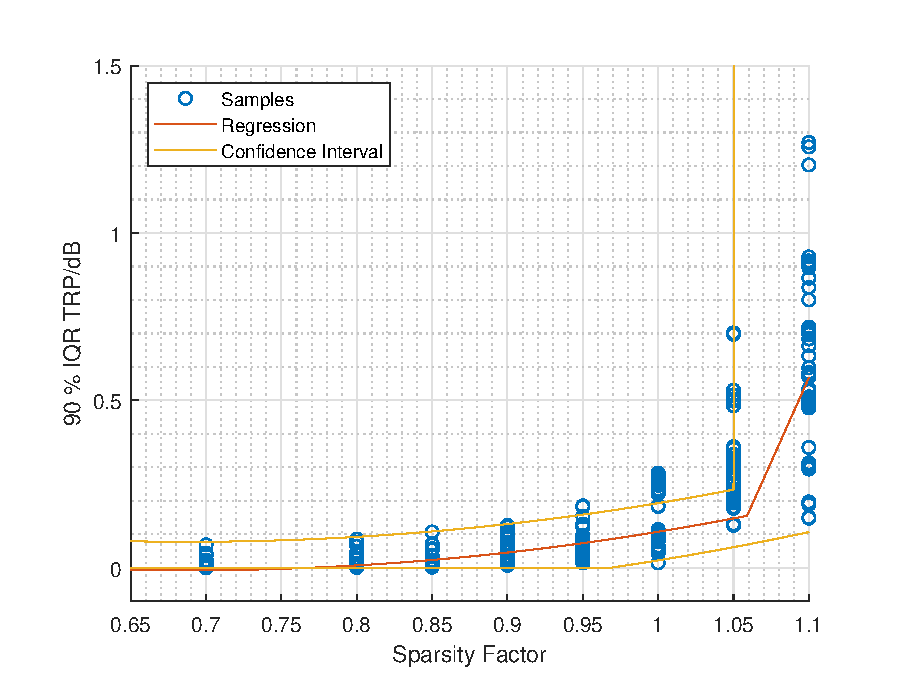
\includegraphics[width=0.49\textwidth]{Matlab/spars-sim7.eps}}
  \centering
  \subfigure[Zoom 2]{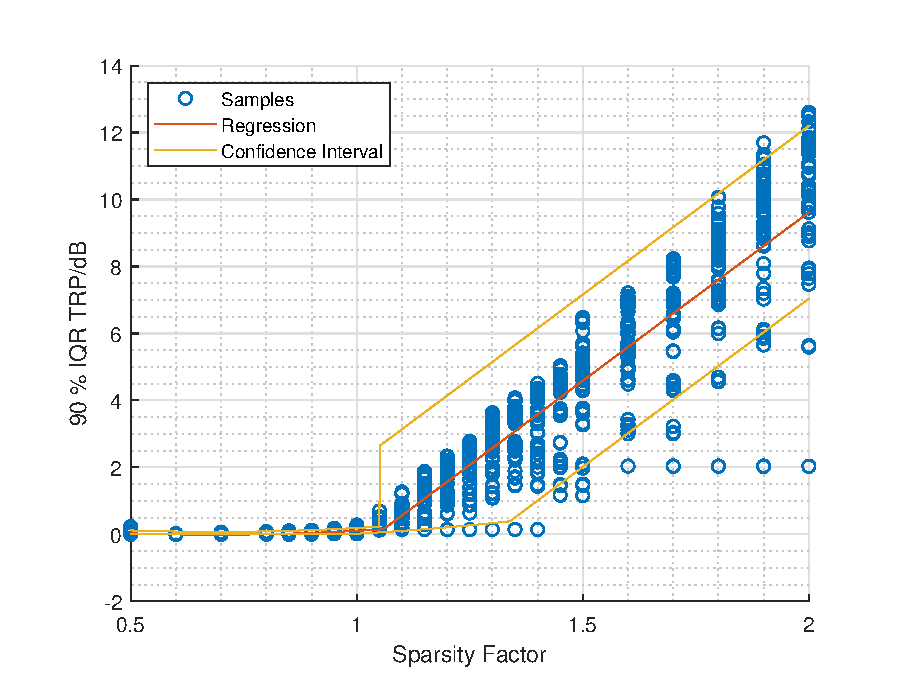
\includegraphics[width=0.49\textwidth]{{Matlab/spars-sim6.eps}}}
\caption{Simulation result over SF}
\label{fig:simressf}
\end{figure}

The marginal probability of the resulting \ac{TRP} \acp{IQR} from the simulation is depicted in fig. \ref{fig:sparssim3}. There are two major areas: Primarily the scattering of the \ac{TRP} is mostly independent from the \ac{SF}. Secondary the \ac{TRP} is dependent from \ac{SF} at around $\text{SF} > 1$. It seems that the \ac{TRP} is mostly independent from all other input parameters.

\subsection{Regression}

The regression of the \ac{TRP} equation is done as described in section \ref{sec:regod} using the parameter matrix $X$ from equation \ref{eq:parammatrix}. The regression is done separately for the two areas. Starting with $\text{SF}\le 1$. With the parameter matrix $X$, the \ac{COD} is $\SI{48}{\percent}$ and the least significant parameter is the interaction between the array sizes with $p = \SI{47}{\percent}$. In the following both array size parameters are also discarded because of their low significance leading to a \ac{COD} of $\SI{48}{\percent}$, with all parameters significant. So the \ac{CTF} has a slight impact on the resulting regression with a coefficient of $b_3=\SI{3.3e-2}{\decibel}$. This corresponds to the maximum introduced additional error of $b_3\cdot\text{CTF}_\text{max}=b_3\cdot 1$, so the error is negligible. Setting $b_3 = 0$ leads to an \ac{COD} of $\SI{42}{\percent}$.\\
Starting the regression of the second area with $\text{SF} > 1$ also with the parameter matrix $X$ leads to a \ac{COD} of $\SI{92}{\percent}$. There the least significant parameter is the \ac{CTF} with $p = \SI{65}{\percent}$. Further stepwise discarding of the least significant parameters leads to a \ac{SF} dependent function with residual dependency to the two dimensional array size. Discarding the array size gives a \ac{COD} of $\SI{84}{\percent}$. Further discarding of the quadratic \ac{SF} parameter has not a big impact and the \ac{COD} is unchanged. The resulting function is thus:

\begin{equation}
\text{TMP}\left(\text{SF}\right)=\begin{cases} 
\SI{0.56}{\decibel}-\SI{1.6}{\decibel}\cdot \text{SF}+\SI{1.2}{\decibel}\cdot\text{SF}^2 & \text{for}\ \text{SF}\le 1.1\\
\SI{-10}{\decibel}+\SI{10}{\decibel}\cdot\text{SF} & \text{for}\ \text{SF}>1.1\end{cases}
\end{equation}

It has been shown that, for the because of the lower error interesting first area, the array size is not significant for the scattering. This proves, that the \ac{CrefA} approach is working. Furthermore it has been shown that the \ac{CTF} has a very little impact on the measurement error and can thereby be neglected, so that with the \ac{CTF} the number of measurement points can be effectively reduced. Also in the second area the \ac{CTF} and the array dimensions are mainly insignificant, which is intended. These findings are also proofed by the marginal probabilities plotted in the annex in the figures \ref{fig:sparssim3} and \ref{fig:sparssimbox}.\\
The marginal probability of the means of each scattering for all parameter combination is plotted in fig. \ref{fig:sparssimboxmean}. The mean of the scatterings of the \ac{TRP} is for $\text{SF} \le 1$ distributed around zero and the value range is always in the vicinity of some $\SI{1e-3}{\decibel}$.\\
The $\SI{95}{\percent}$ confidence interval of the regression is plotted in fig. \ref{fig:simressf} in yellow. It is computed as in equation \ref{eq:conv} described. It is also split in two parts.

\subsection{Comparison of Different Reference Angles}

The same simulation is carried out by using the reference angle introduced by \cite{hansen} in equation \ref{eq:refahansen}. The resulting marginal probability distribution is plotted in fig. \ref{fig:sparssimboxhansen}. Because of the tendencially smaller sampling interval, refer to fig. \ref{fig:evolvpattern3}, the \ac{IQR} of the \ac{TRP} distributions is lower. This leads to a unnecessary high sampling density. Also the regression parameters show that a residual dependency is present, combined with a lower coefficient of determination as in the \ac{CrefA} sampling density approach from above:\\
For $\text{SF}\le 1$, starting with the regression from equation \ref{eq:parammatrix}, the significant parameters are the \ac{CTF}, the number of elements in $y$ and the \ac{SF} with a \ac{COD} of $\SI{24}{\percent}$. Discarding all parameters except the \ac{CTF} leads to a \ac{COD} of $\SI{21}{\percent}$, so the \ac{TRP} \ac{IQR} is mainly independent from \ac{SF}.\\
For $\text{SF}\ge 1$, starting with the regression from equation \ref{eq:parammatrix}, the significant parameters are the number of elements in $y$, the number of elements in $z$ and the \ac{SF} with a \ac{COD} of $\SI{71}{\percent}$. Discarding the array size parameters leads to a \ac{COD} of $\SI{54}{\percent}$, showing the significant residual correlation between array size and \ac{TRP} \ac{IQR}.\\
A similar outcome is recognised using the reference angle from \cite{2018arXiv180310993F}, where the reference angle increment is computed by formula \ref{eq:hansenrefa}. To generate the sampling angle the reference angle is multiplied by \ac{SF} and provided that the resulting angle increment is less than $\SI{15}{\degree}$. This results for small arrays in unnecessary fine sampling. Regarding fig. \ref{fig:sparssimboxericsson}, showing that for small arrays the \ac{IQR} scattering is independently low. That can also be proofed by regression. For $\text{SF}\ge 1$ the significant parameters are the numbers of elements in $z$ and the area of the array with a \ac{COD} of $\SI{73}{\percent}$. Discarding the array size parameters leads to a \ac{COD} of $\SI{44}{\percent}$, whereby it is with \ac{CrefA} implementation $\SI{84}{\percent}$.

\subsection{Comparison of CSSG and CDG}

\begin{figure}[h]
\centering
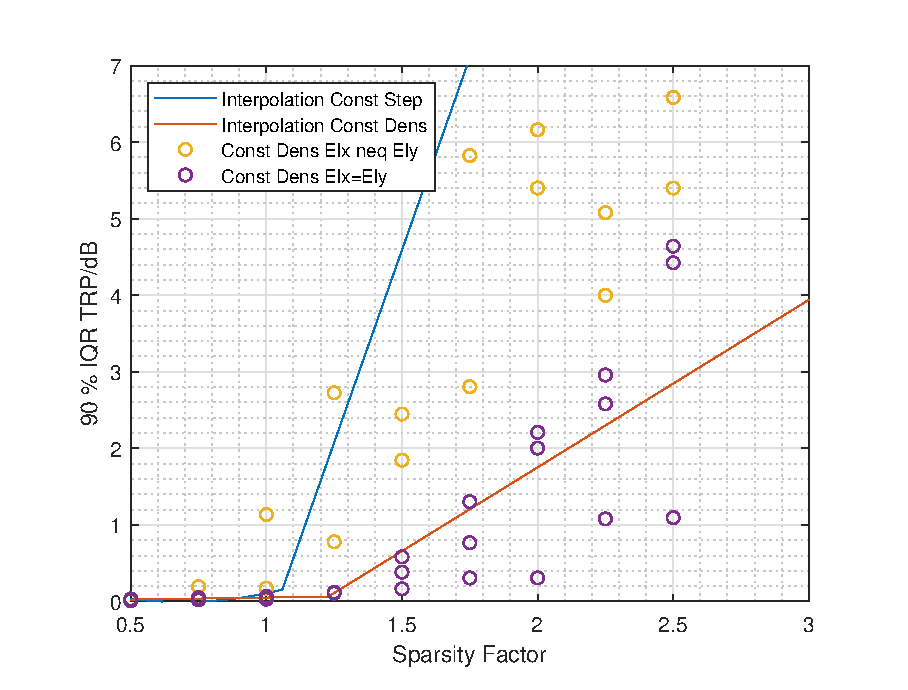
\includegraphics[width=0.49\textwidth]{Matlab/spars-sim3.eps}
\caption{The CDG compared to the CSSG}
\label{fig:cdg}
\end{figure}

The computational effort for \acp{CDG} is with this implementation very high, caused by the fine $\SI{0.2}{\degree}$ sampling grid. Therefore less samples are computed. The result is depicted in fig. \ref{fig:cdg}. It is shown, that for uniform arrays the performance of the \ac{CDG} is better than the \ac{CSSG}. For non uniform arrays the performance equal to a \ac{CSSG}. This is caused e.q. for a not quadratic array by unnecessary high sampling density in azimuth and sparse sampling in elevation caused by the non-adaptive \ac{CDG}. This leads for the same number of points to a similar or worse result. In addition, using the \ac{CTF}, the number of measurement points is even lower for the \ac{CSSG}.




\chapter{Measurement Distance}

\section{Simulation}

\section{Measurement}
\chapter{Conclusion} \label{chap:8}

The achieved findings of this work shall be described in this chapter. Furthermore, an outlook for future work will be drawn.

\section{Achievements}
This work presents a coexistence testing solution for devices with or without antenna ports, based on a novel regulatory test system that has a compact size and high quality shielding and allows lower coupling losses. The project implements normalized and conducted measurements to perform the device-testing, and investigates the MU for both cases. To this end, an algorithm for the optimization of antenna pairs is implemented on both the simulation and the measurements. After that, the hardware and software implementations for PSD and receiver blocking test cases are done based on the standard (link). The results for both single and multi-antennas DUTs showed that comparable MU results to the conducted measurements can be achieved by the normalized approach. While studying the MU results for the presented test cases, many factors may influence the accuracy of the test results. In addition to the errors caused by thermal noise, there are interferences and cross-talk between the measurement antennas that can influence the results. Also, the results of the MU for single-antennas DUT are proved to be better than those of multi-antennas. Finally, in-band testing determines the performance of wireless devices and the thresholds where wireless communications are degraded as well as the threshold where communications stop i.e where the limits set by the standards are exceeded. The report of these tests provides the necessary data to make a more informed risk analysis of the radio?s behavior and to enable troubleshooting the reported interference problems. The results prove that performing the normalized OTA measurements doesn?t result in a major degrading the quality of the evaluation.
Further investigations and research are possible to improve this work; for the selection of best probe antennas within the test chamber, the simulation can be improved by including other effects that can increase the accuracy of the simulation to match the choice based on actual measurements such as minor reflections in the chamber and isolation between the probe antennas (link).


\section{Outlook}


% Ab hier beginnt der Anhang
%\appendix
%\addcontentsline{toc}{chapter}{Anhang}

%\addcontentsline{toc}{chapter}{Index}
%\printindex

%\addcontentsline{toc}{chapter}{Literaturverzeichnis}

% Haben Sie das "biblatex"-Paket nicht installiert, benutzen Sie folgendes:
% Ohne das "biblatex"-Paket (s. bericht.sty) produziert folgendes
% "deutsche" Zitate in Literaturverzeichnissen gemaß der Norm DIN 1505,
% Teil 2 vom Jan. 1984.
% Die Zitatmarken werden alphabetisch nach Verfassern
% sortiert und sind durch abgekürzte Verfasserbuchstaben plus
% Erscheinungsjahr in eckigen Klammern gekennzeichnet.

% \bibliographystyle{alphadin}
% \bibliography{literatur}

%%%%%%%%%%%%%%%%%%%%%%%%%%%%%%%%%%%%%%%5
% BIBLATEX
% Benutzt man das "biblatex"-Paket, muß man folgendes schreiben:
%\def\refname{Literaturverzeichnis}
%\printbibliography
\printbibliography
%%%%%%%%%%%%%%%%%%%%%%%%%%%%%%%%%%%%%%%5



\chapter{Annex}

This appendix gathers the measurement results of the main scenarios investigated
for the thesis. 

\begin{figure}[H]
     \subfigure{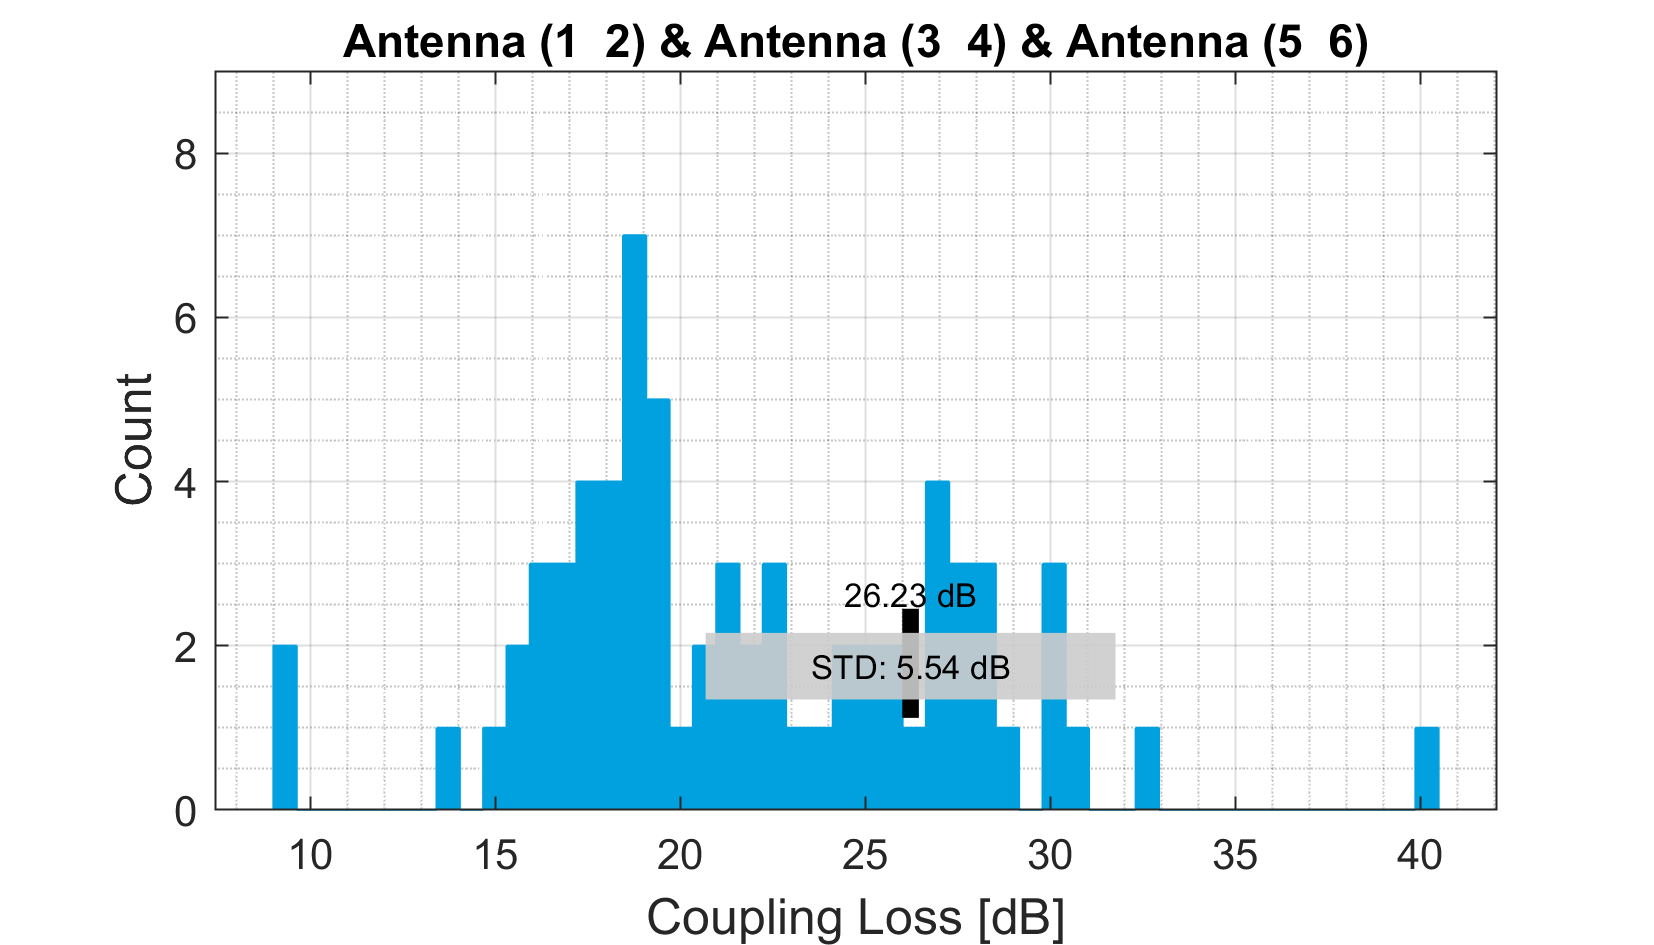
\includegraphics[scale = 0.37]{/Annex/Manual/plot1.png}} 
     \subfigure{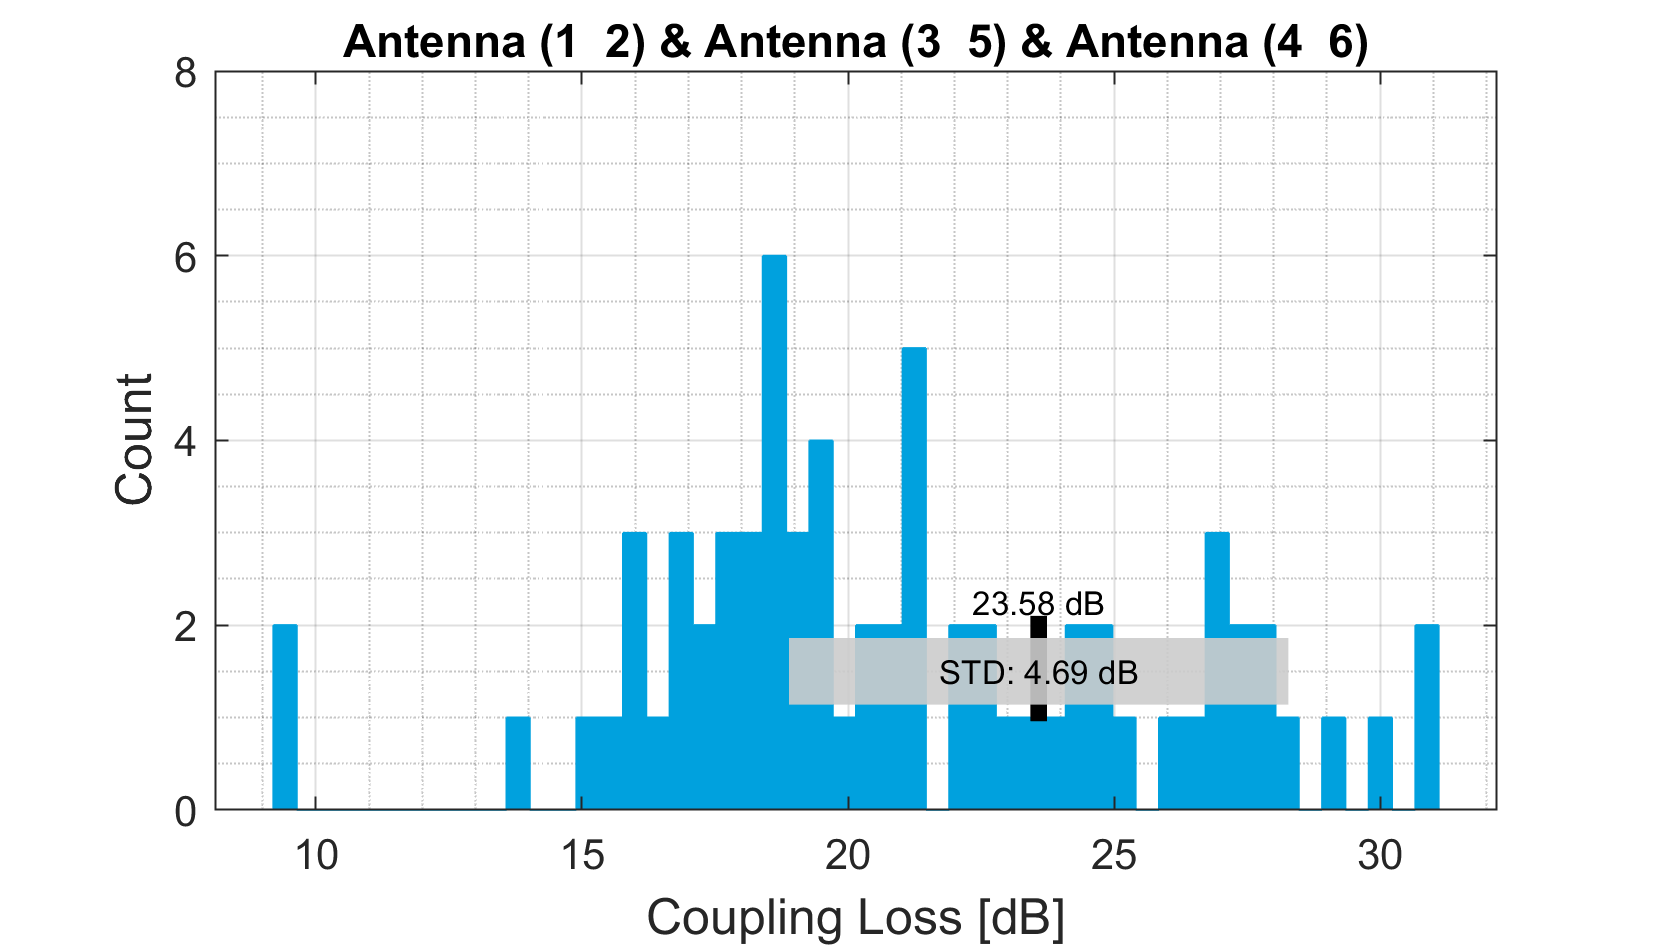
\includegraphics[scale = 0.37]{/Annex/Manual/plot2.png}} 
     \subfigure{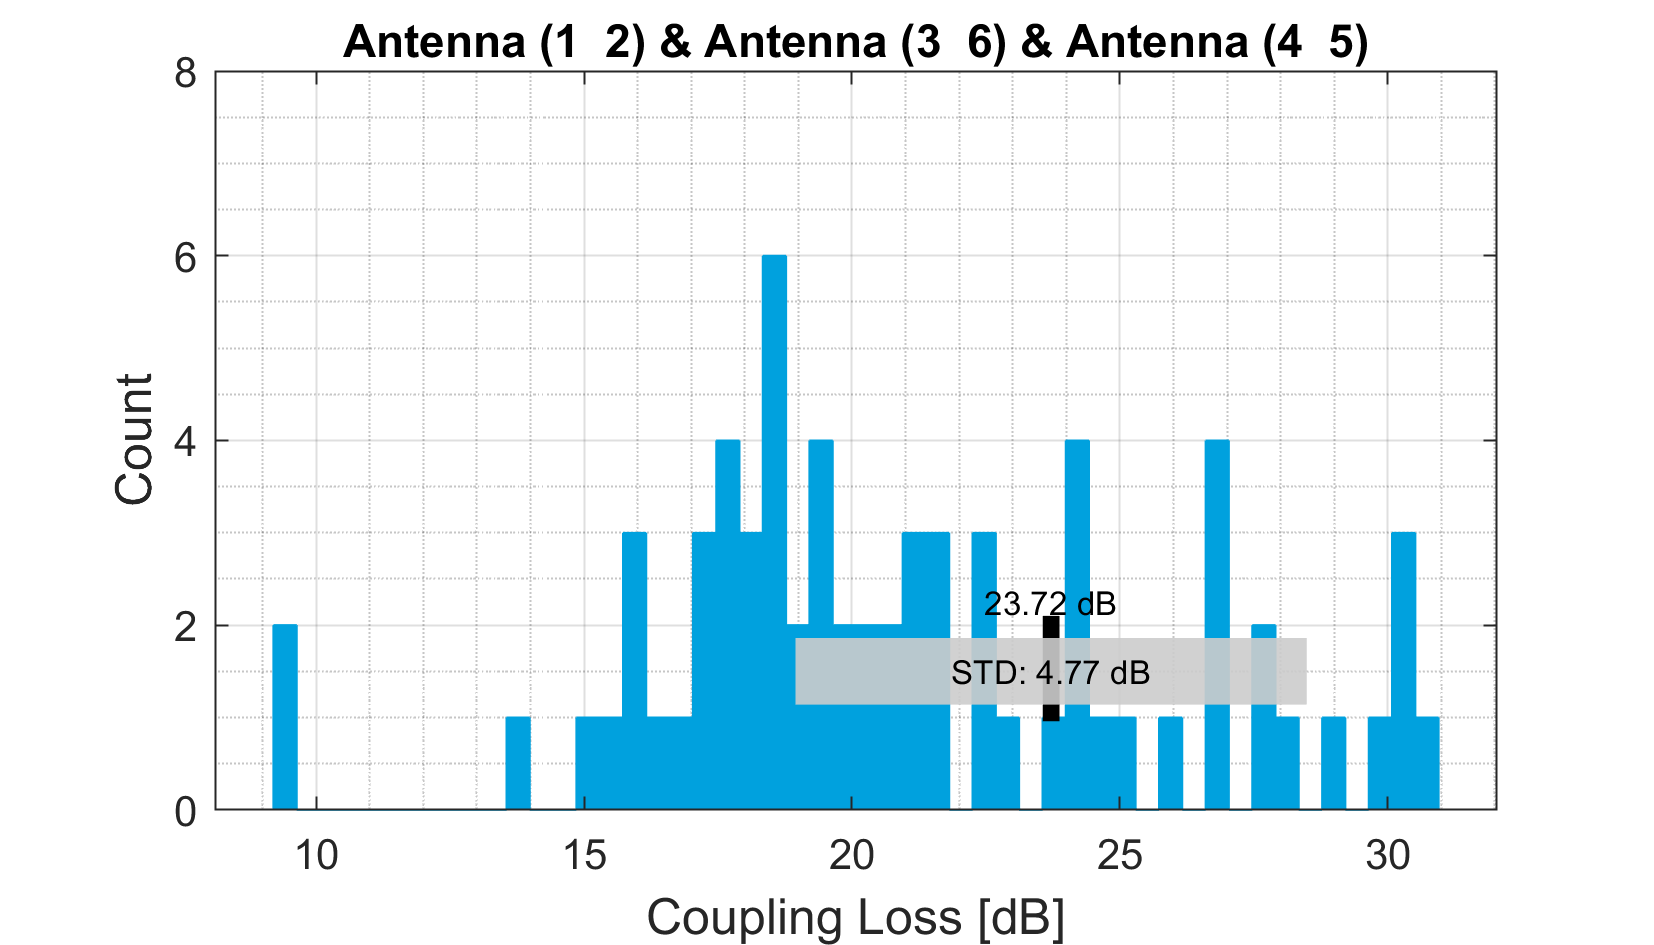
\includegraphics[scale = 0.37]{/Annex/Manual/plot3.png}}  \\
     \subfigure{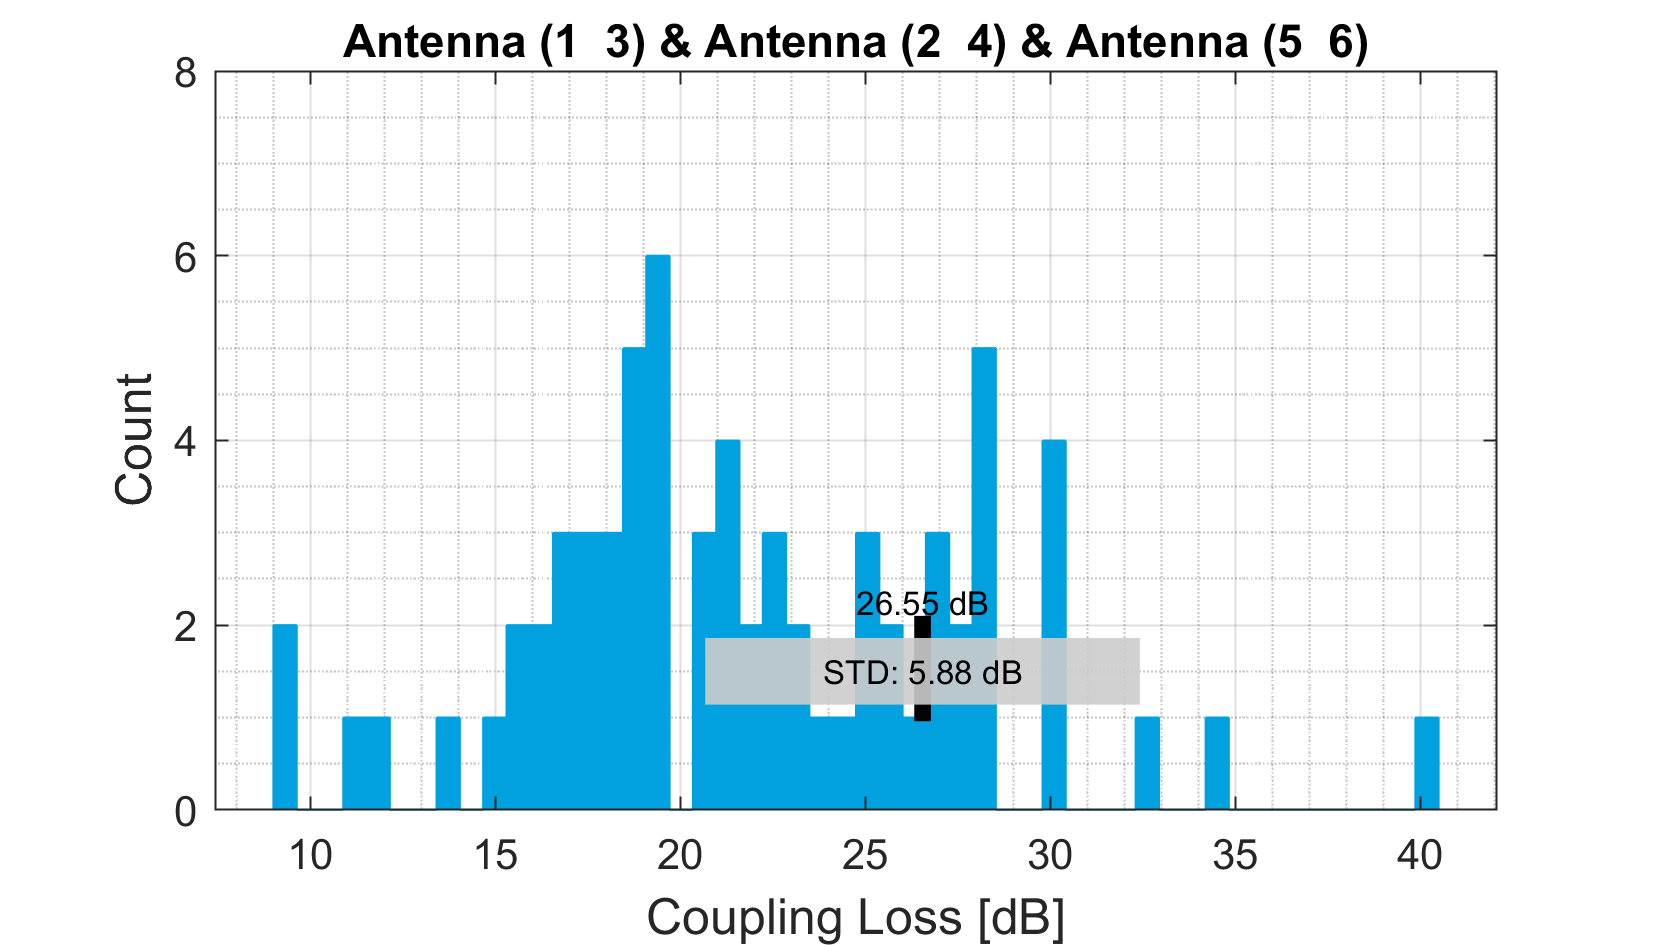
\includegraphics[scale = 0.37]{/Annex/Manual/plot4.png}} 
     \subfigure{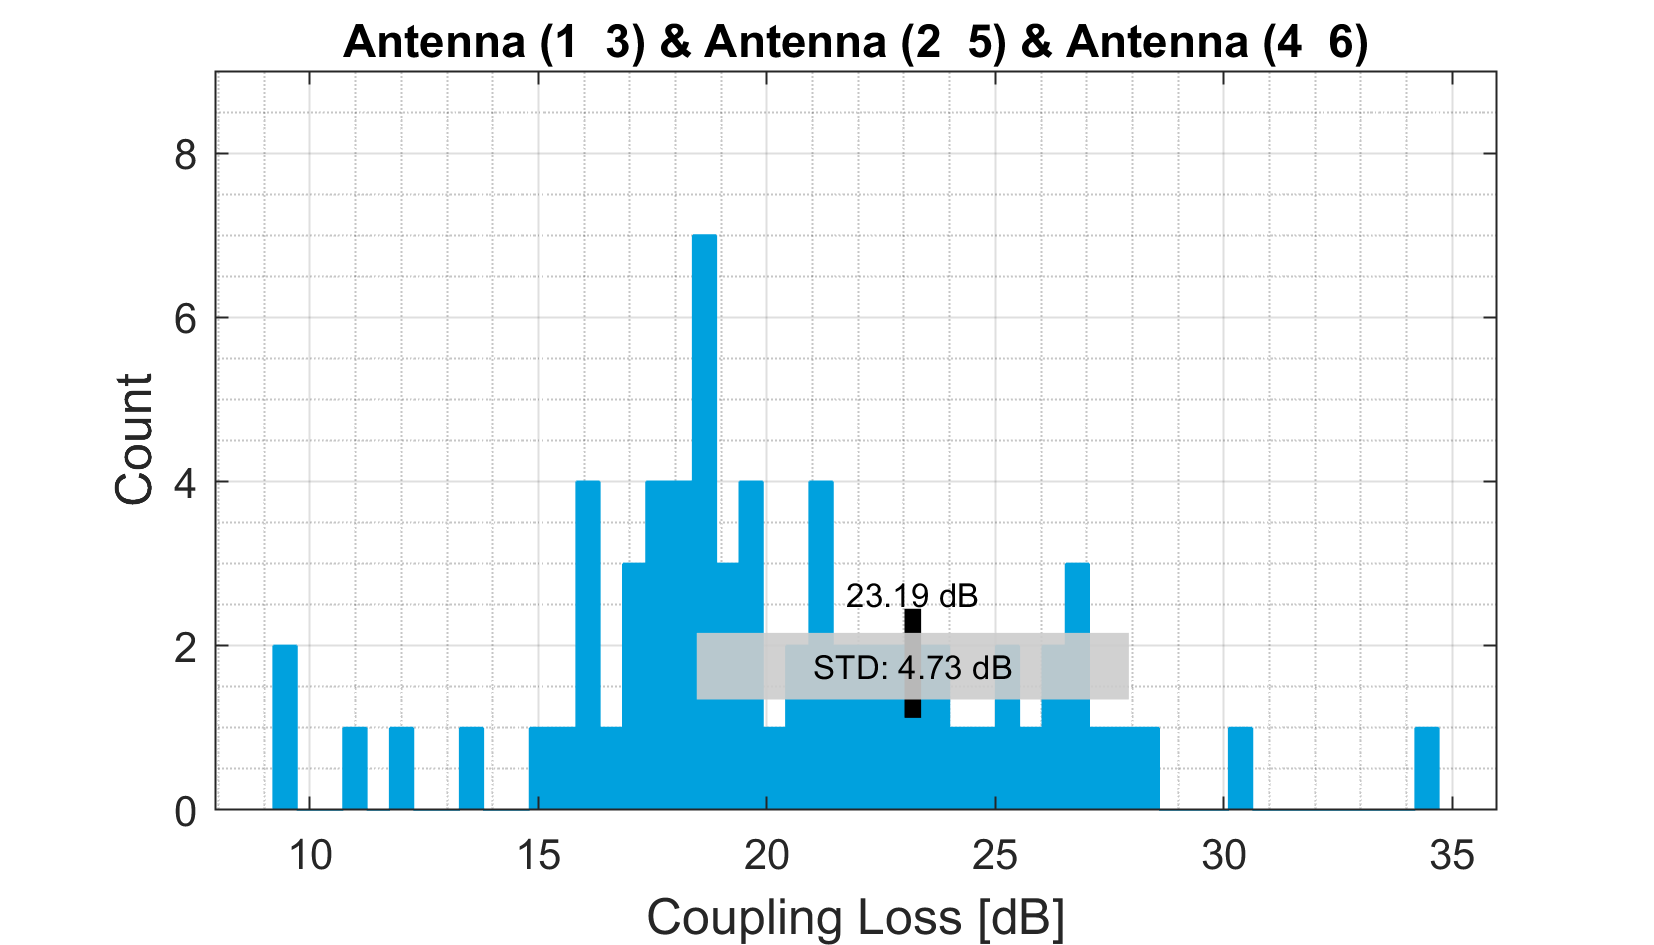
\includegraphics[scale = 0.37]{/Annex/Manual/plot5.png}} 
     \subfigure{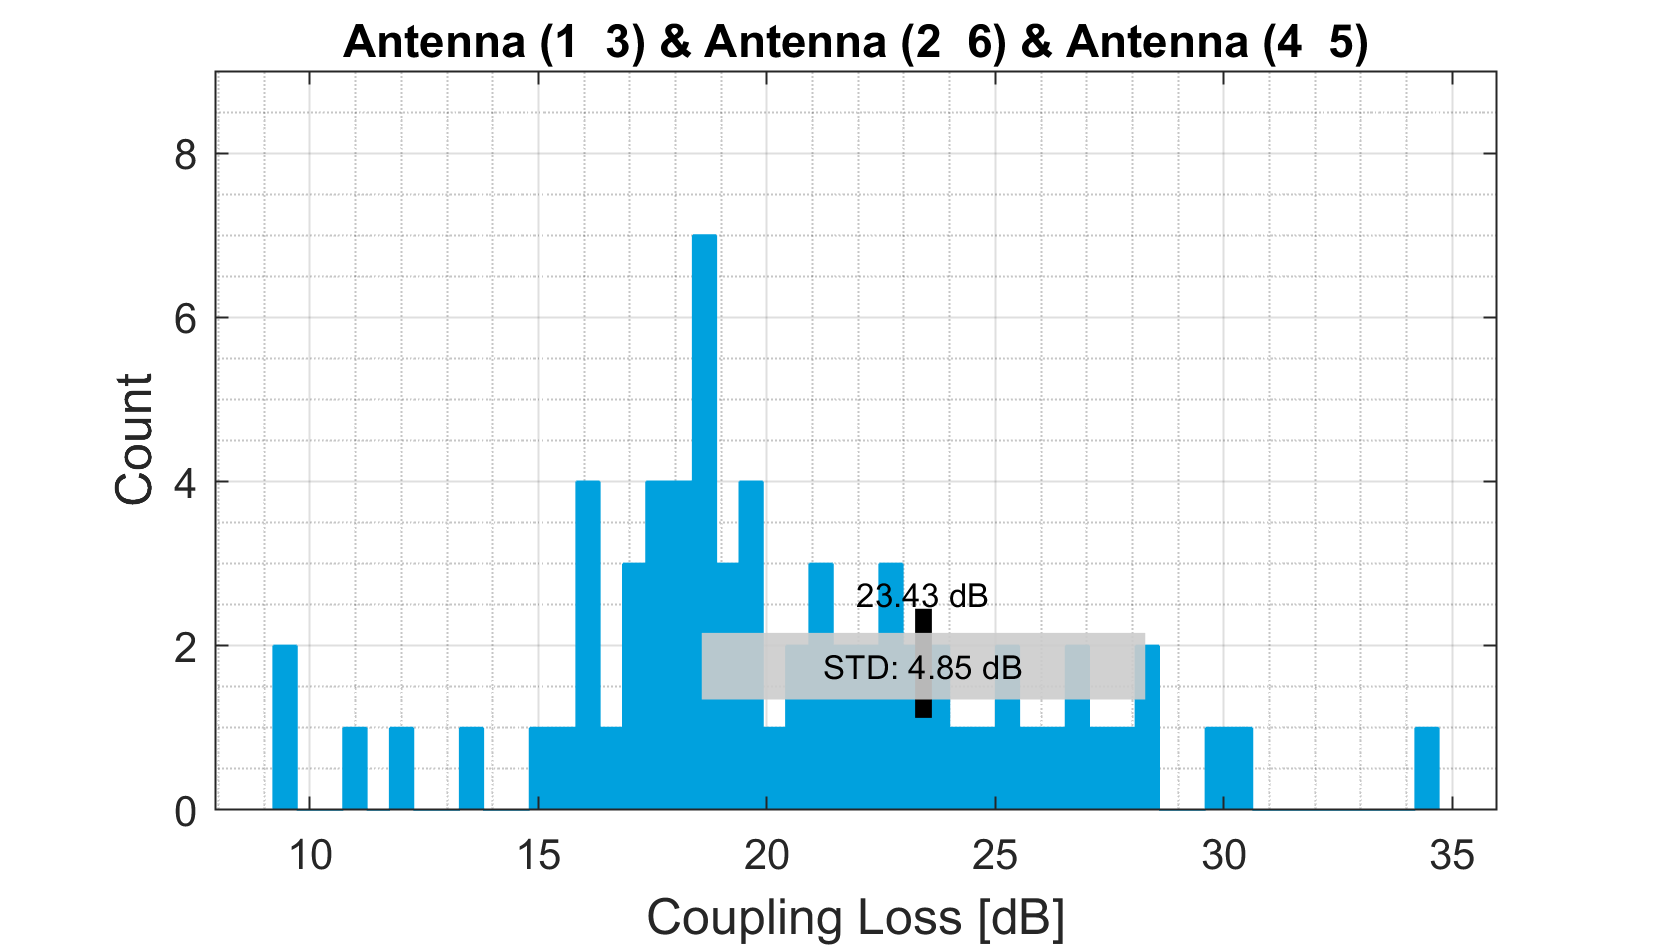
\includegraphics[scale = 0.37]{/Annex/Manual/plot6.png}}  \\
     \subfigure{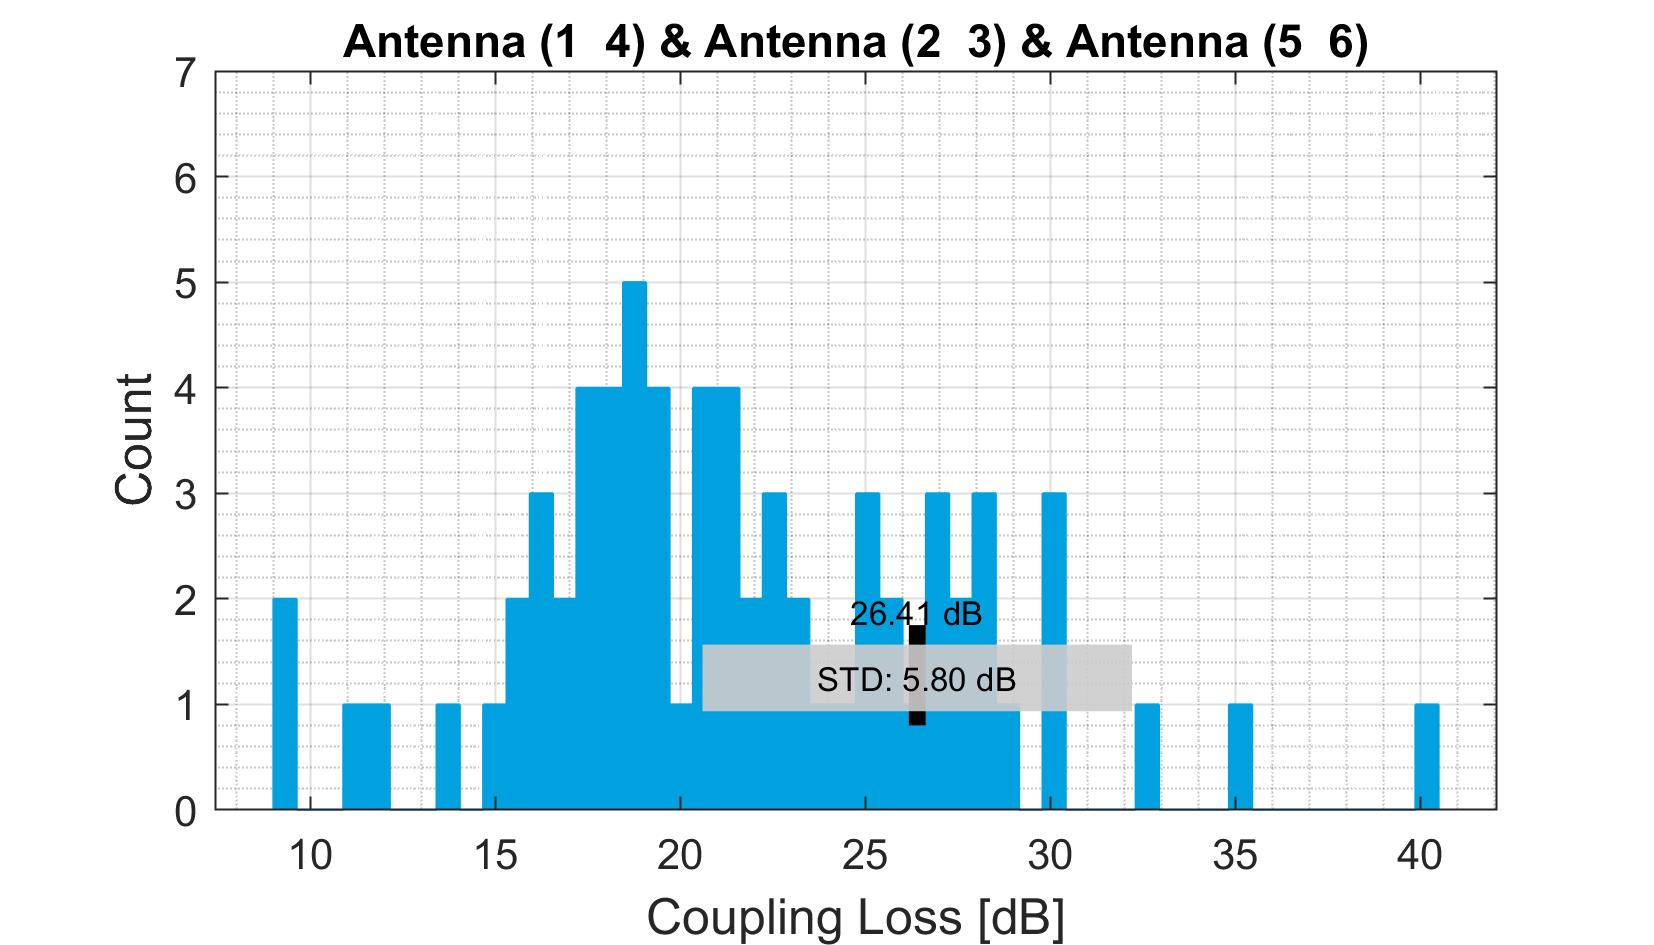
\includegraphics[scale = 0.37]{/Annex/Manual/plot7.png}} 
     \subfigure{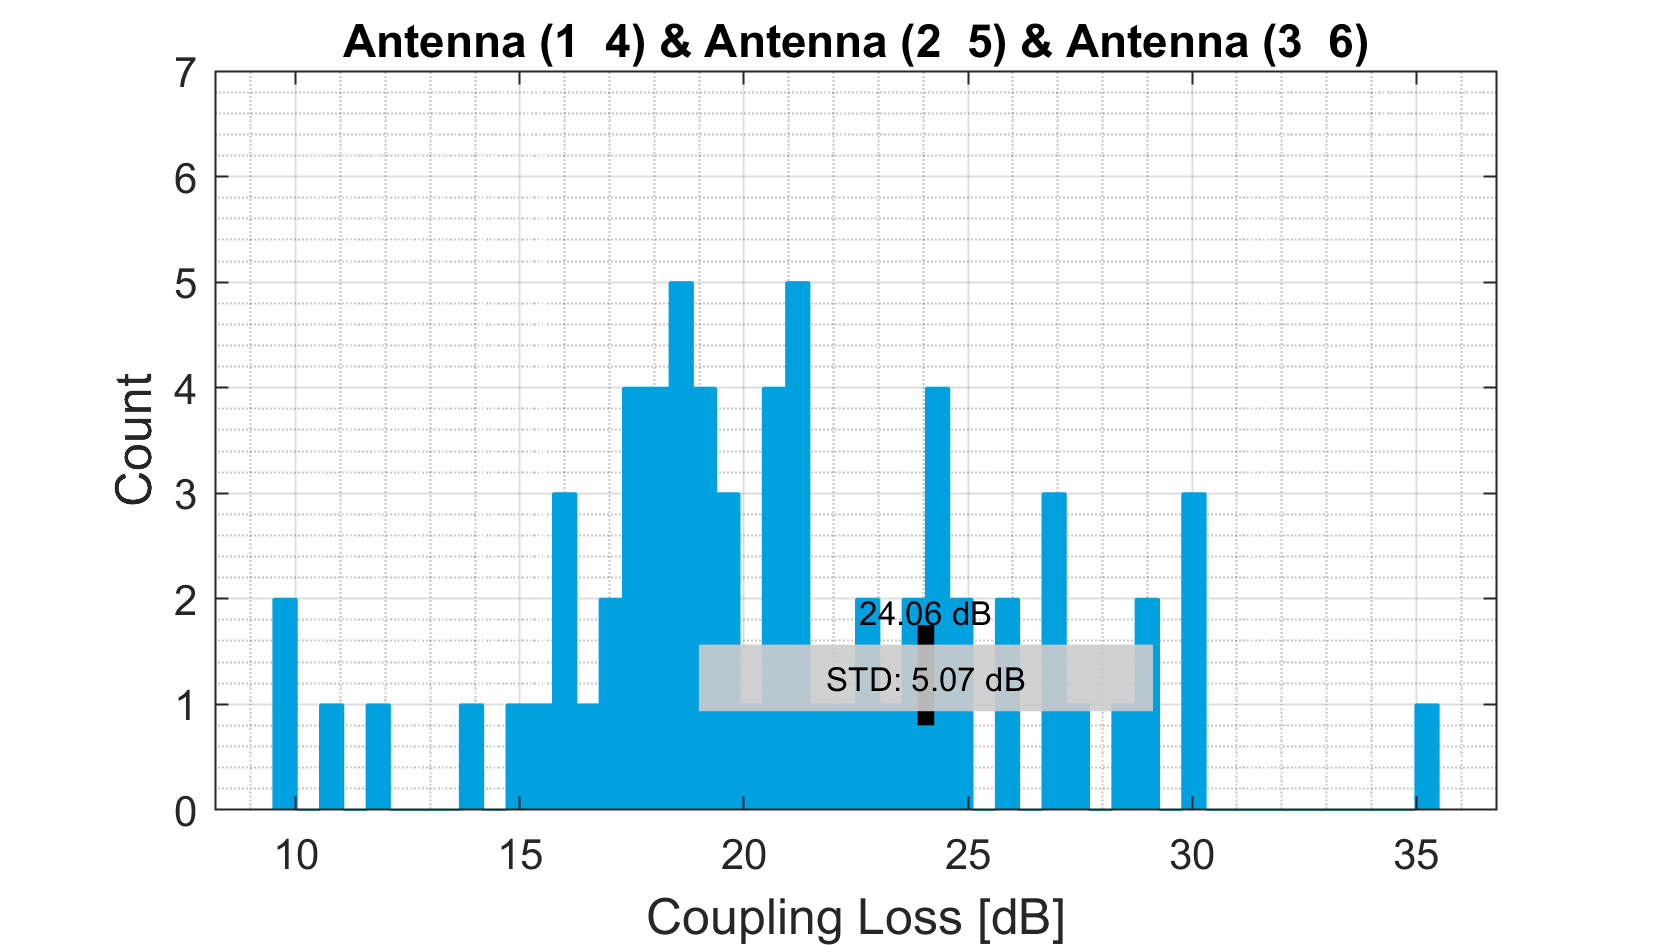
\includegraphics[scale = 0.37]{/Annex/Manual/plot8.png}} 
     \subfigure{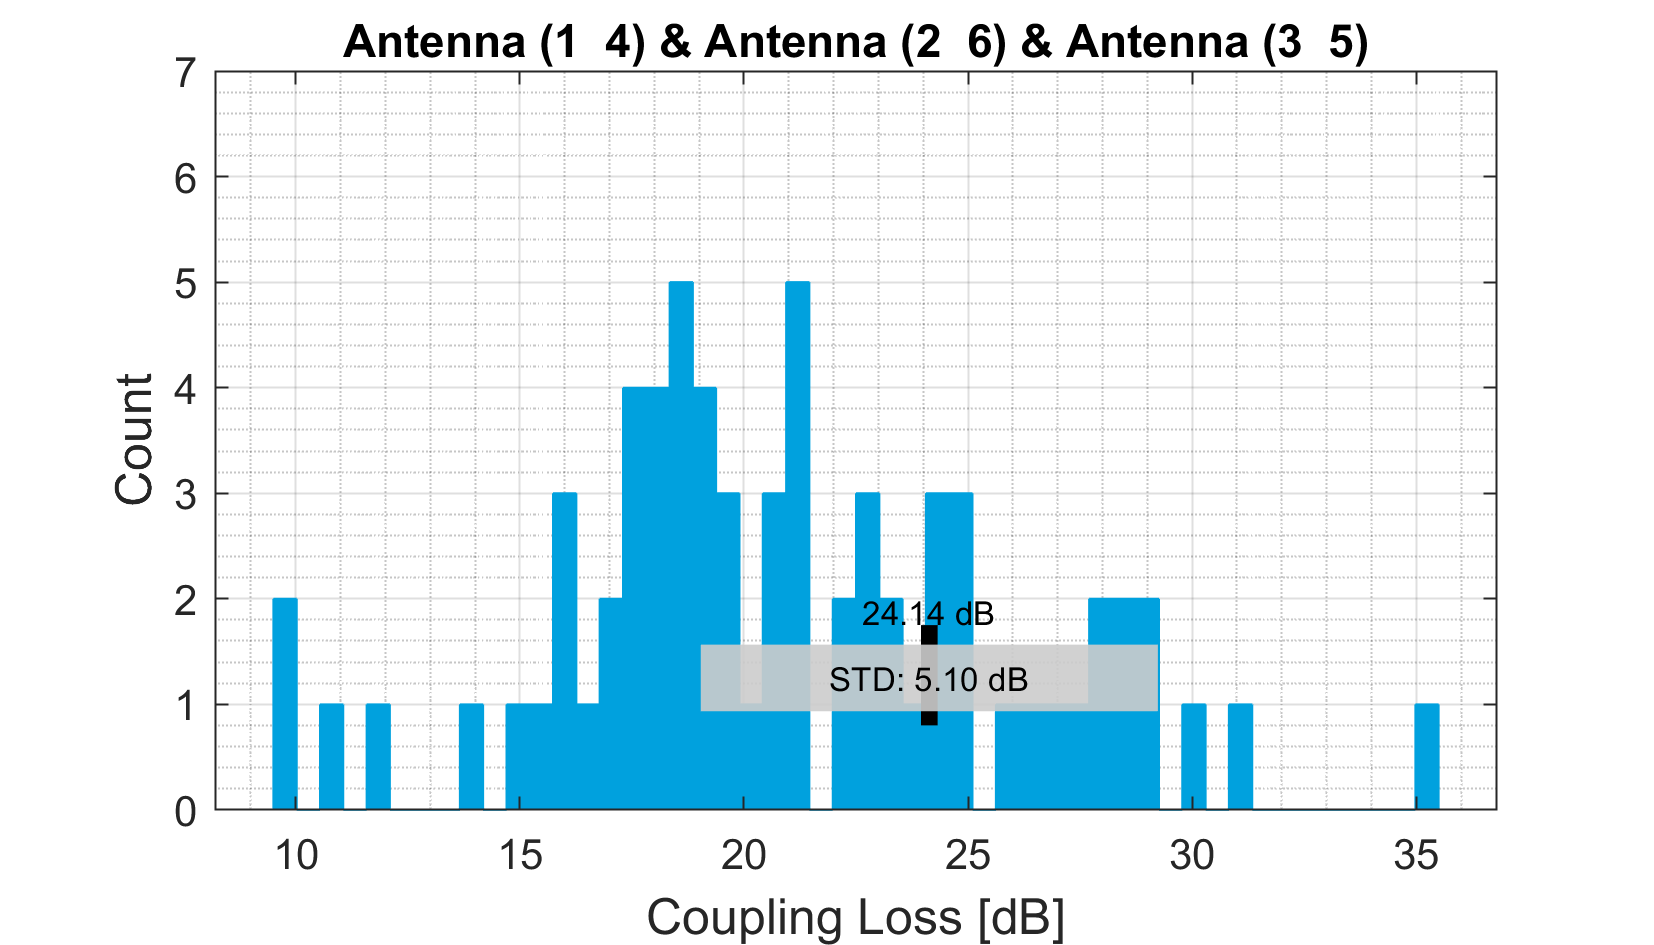
\includegraphics[scale = 0.37]{/Annex/Manual/plot9.png}}  \\
     \subfigure{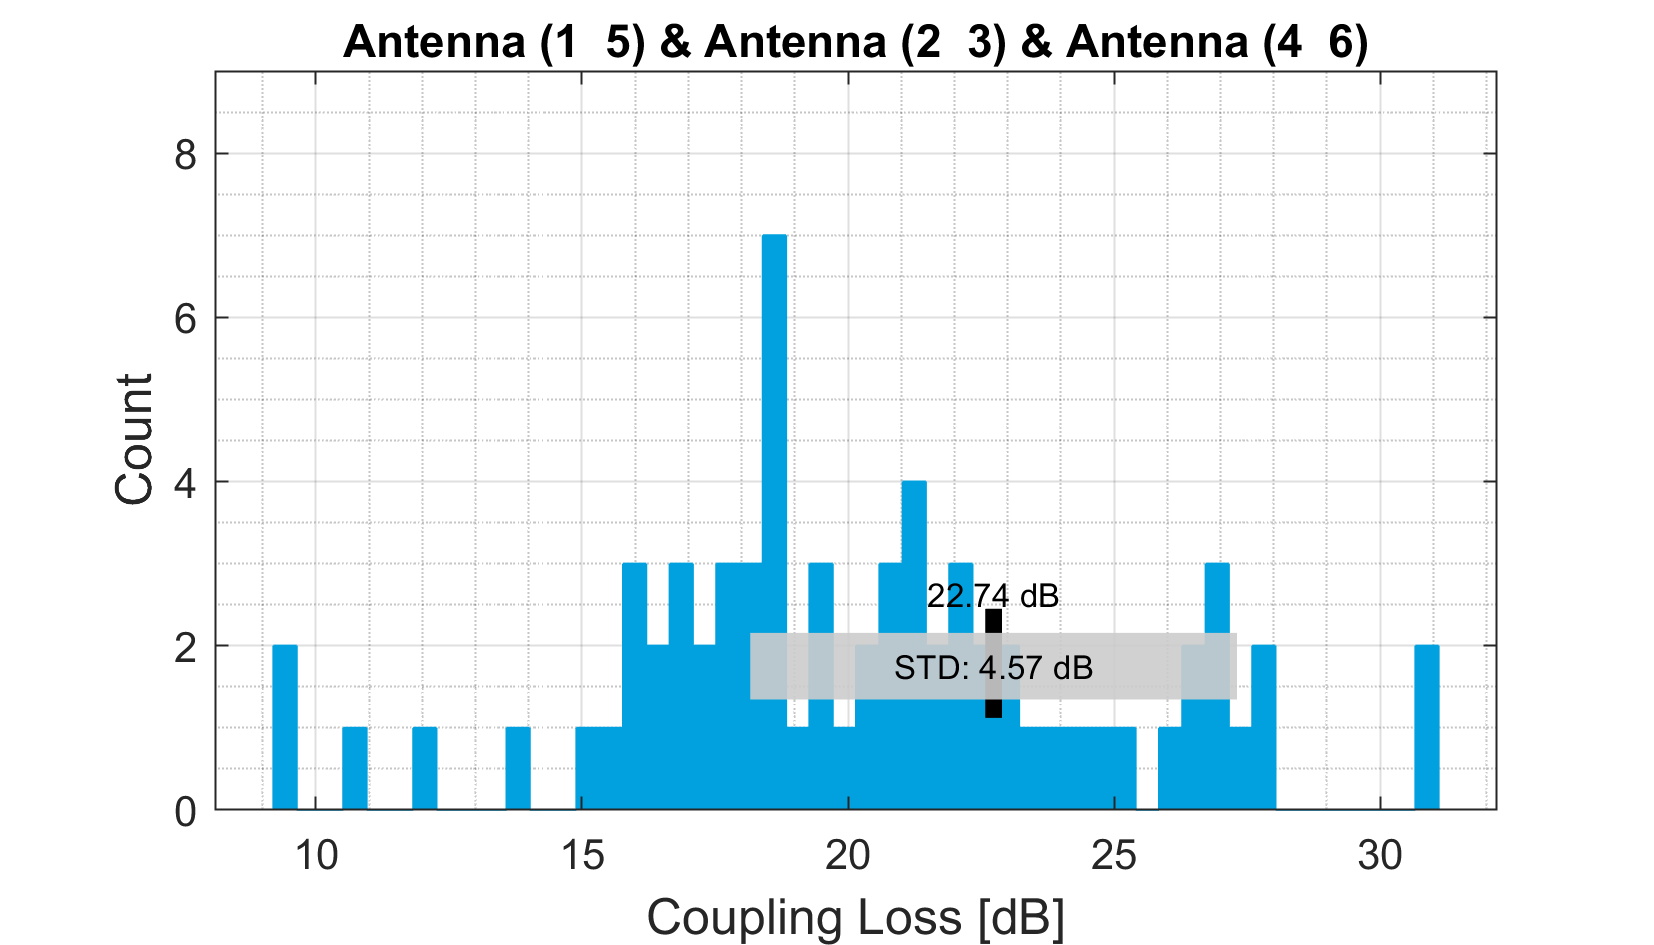
\includegraphics[scale = 0.37]{/Annex/Manual/plot10.png}} 
     \subfigure{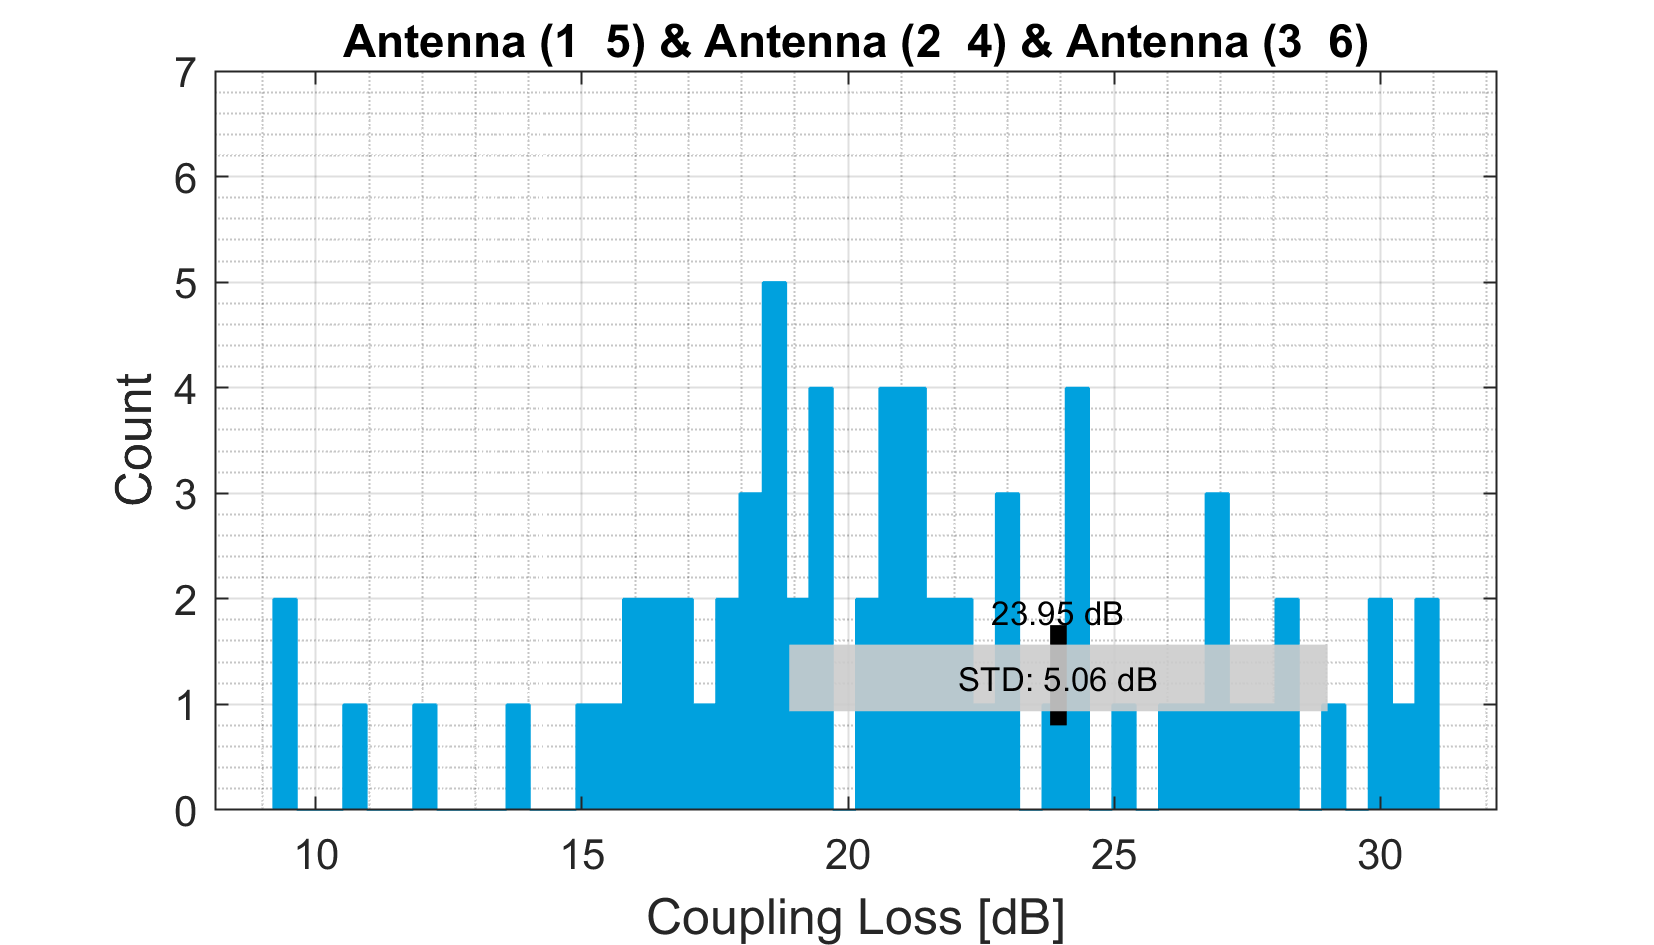
\includegraphics[scale = 0.37]{/Annex/Manual/plot11.png}} 
     \subfigure{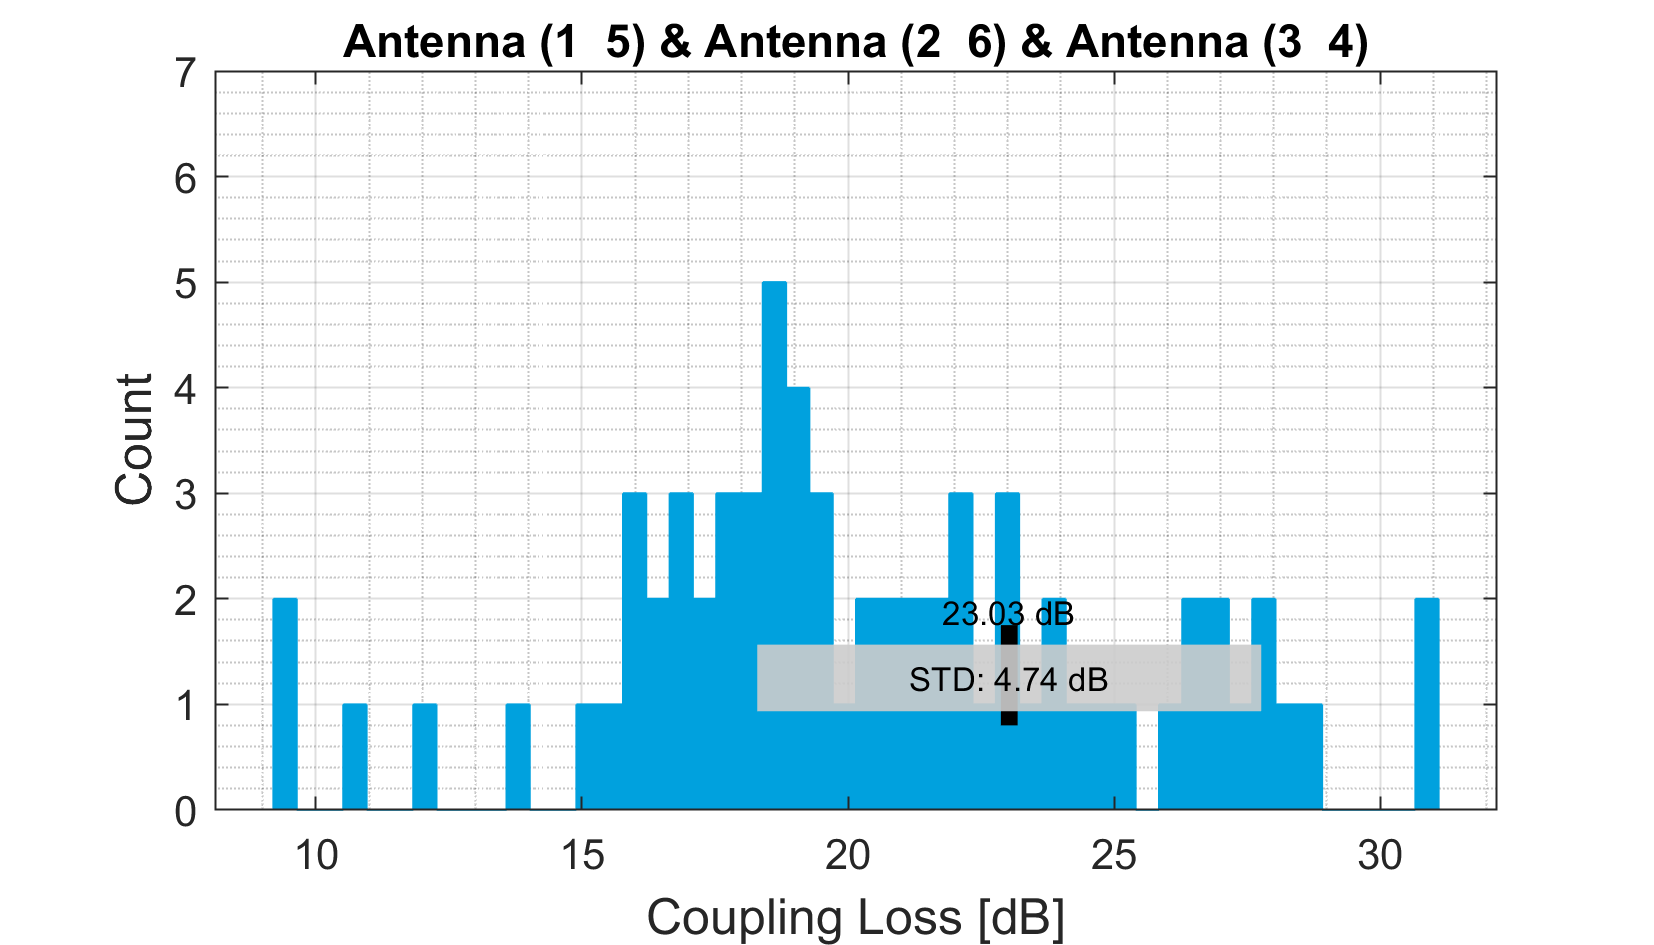
\includegraphics[scale = 0.37]{/Annex/Manual/plot12.png}}  \\
      \subfigure{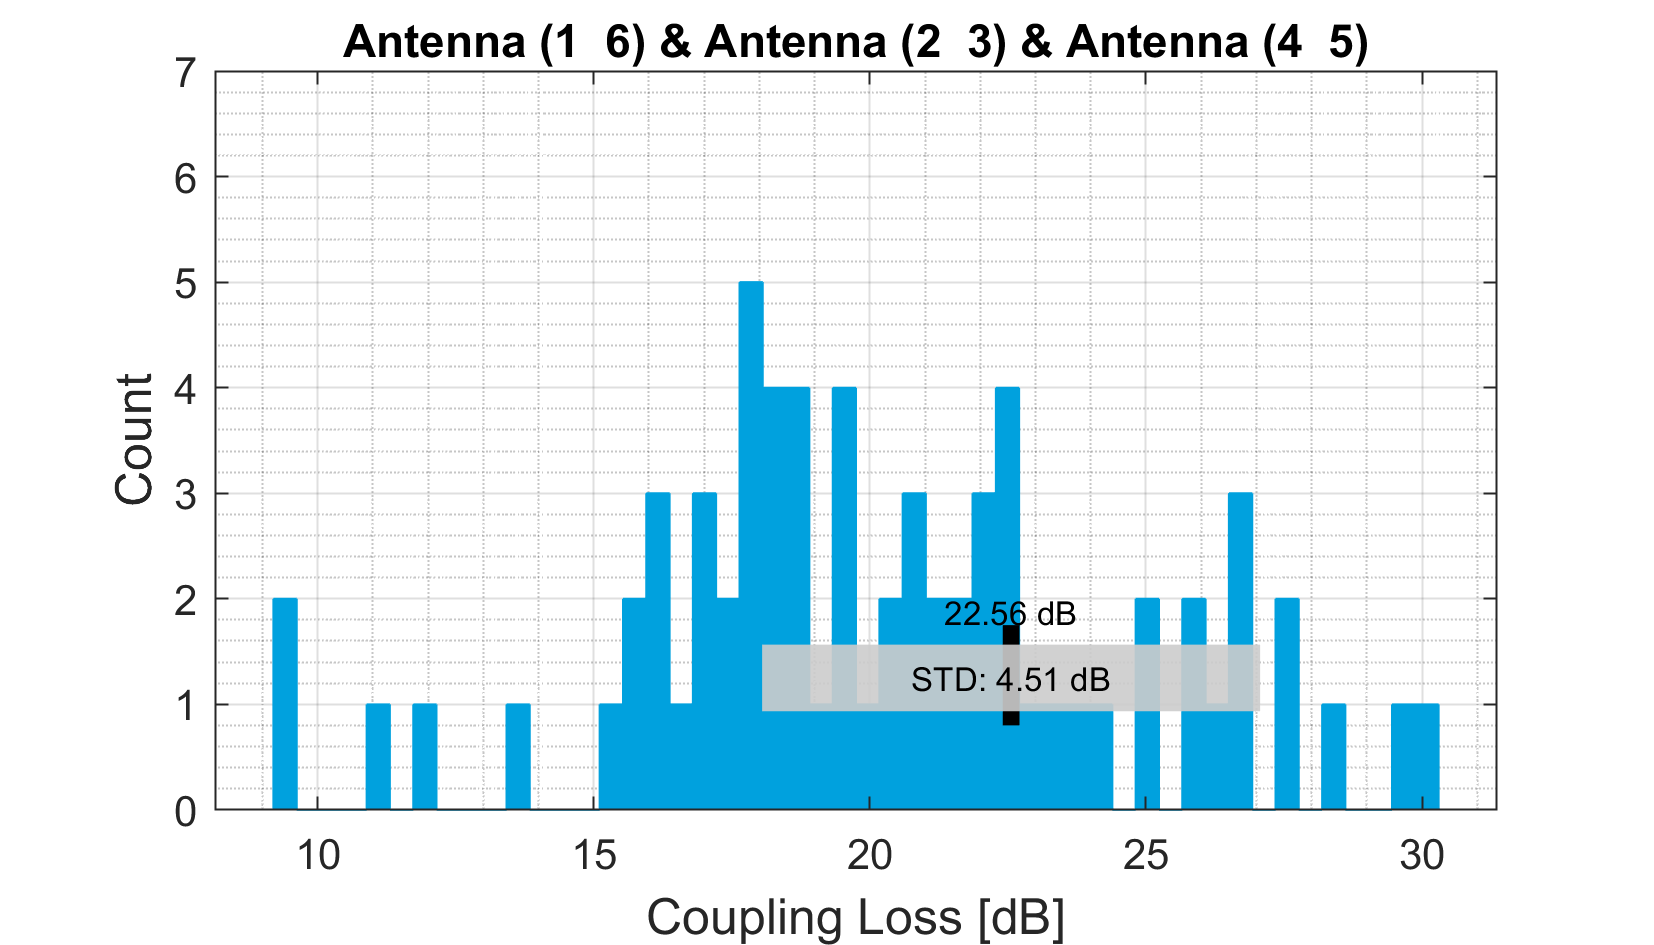
\includegraphics[scale = 0.37]{/Annex/Manual/plot13.png}} 
     \subfigure{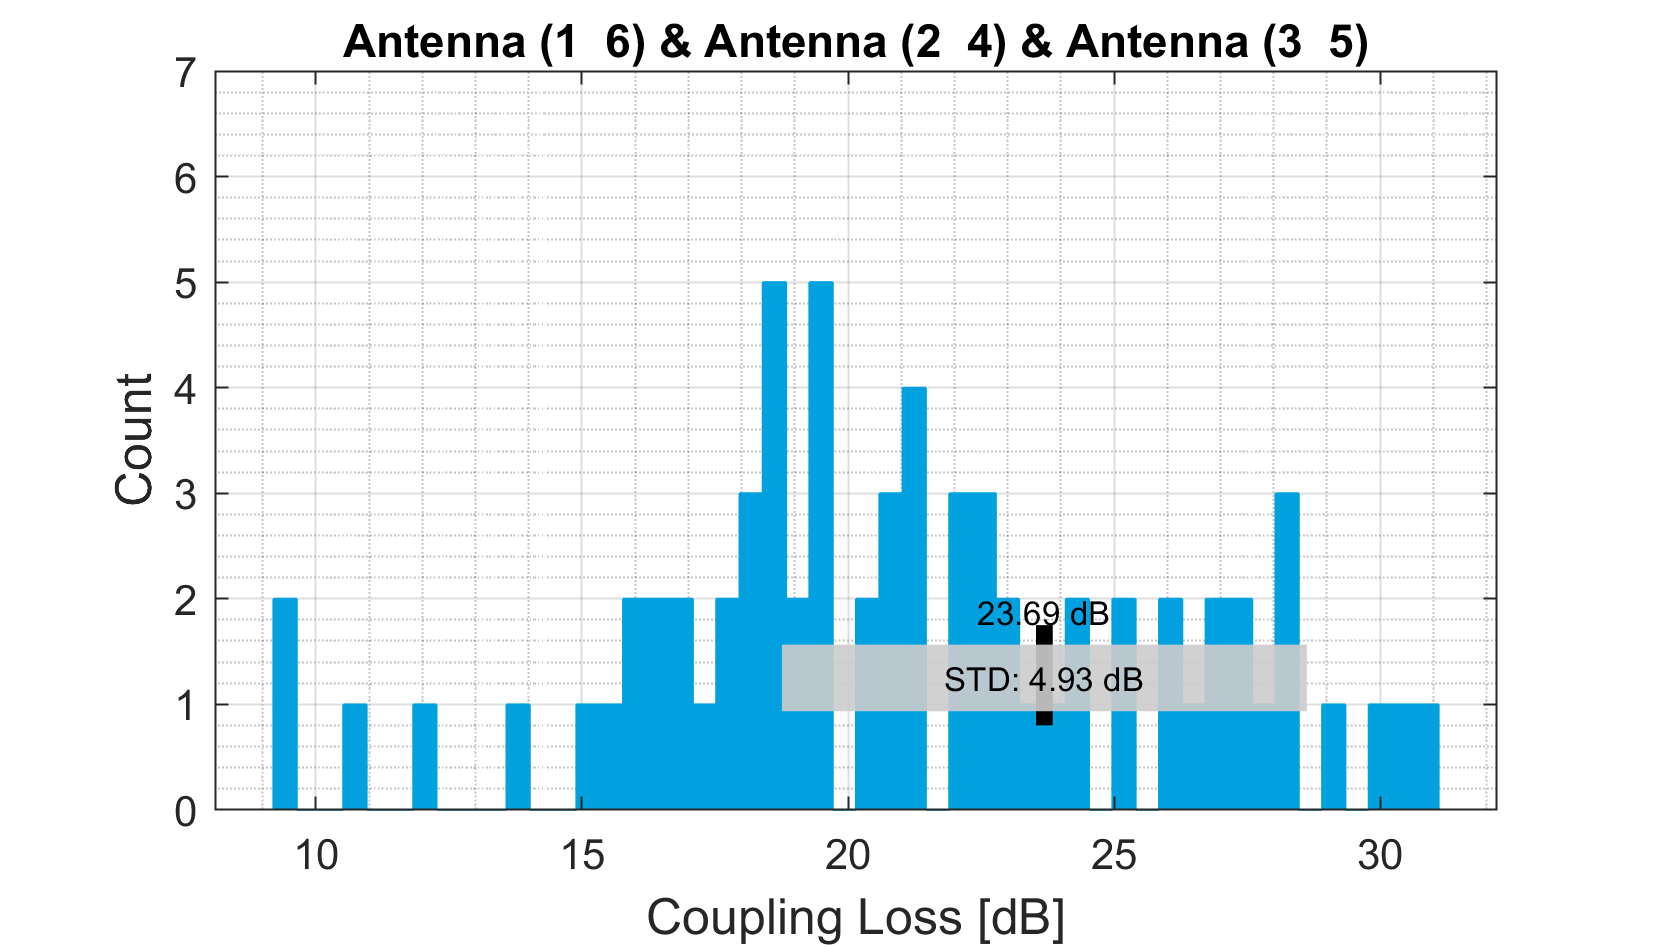
\includegraphics[scale = 0.37]{/Annex/Manual/plot14.png}} 
     \subfigure{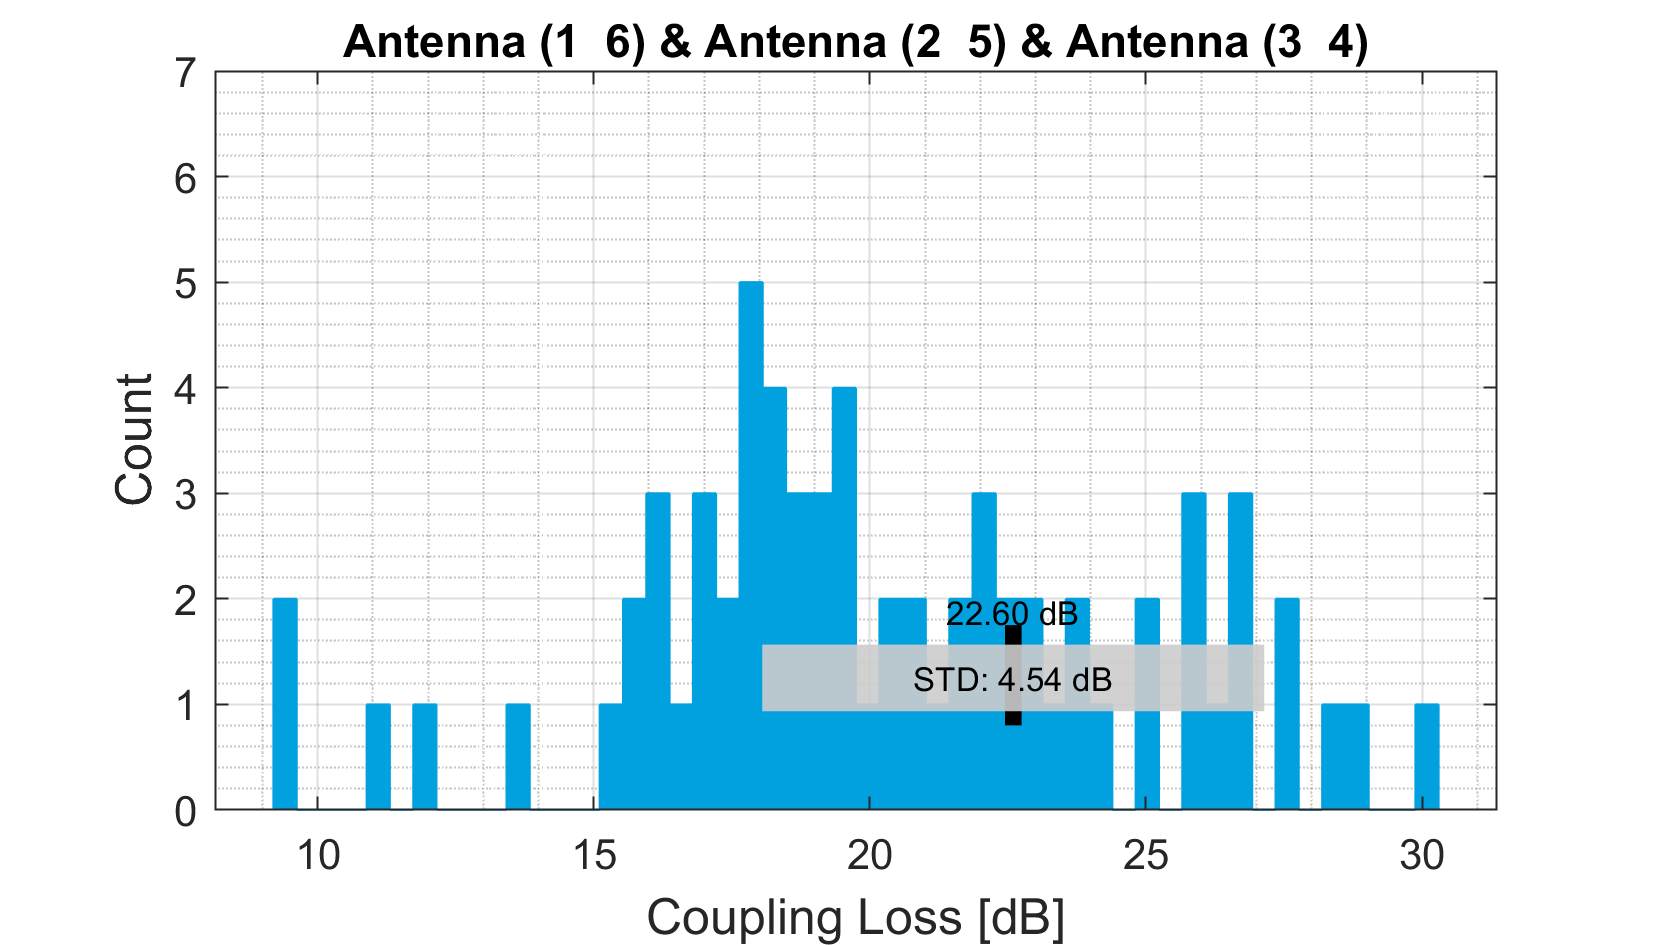
\includegraphics[scale = 0.37]{/Annex/Manual/plot15.png}}  
        \caption{Manual Measurements for optimization of antenna pair}
        \label{fig:three graphs}
\end{figure}






\begin{singlespace}

%\include{changelog}

\newpage
\addcontentsline{toc}{chapter}{Liste der ToDo's}
\listoftodos[Liste der ToDo's]

\end{singlespace}
\end{document}
